
% Default to the notebook output style

    


% Inherit from the specified cell style.




    
\documentclass[11pt]{article}

    
    
    \usepackage[T1]{fontenc}
    % Nicer default font (+ math font) than Computer Modern for most use cases
    \usepackage{mathpazo}

    % Basic figure setup, for now with no caption control since it's done
    % automatically by Pandoc (which extracts ![](path) syntax from Markdown).
    \usepackage{graphicx}
    % We will generate all images so they have a width \maxwidth. This means
    % that they will get their normal width if they fit onto the page, but
    % are scaled down if they would overflow the margins.
    \makeatletter
    \def\maxwidth{\ifdim\Gin@nat@width>\linewidth\linewidth
    \else\Gin@nat@width\fi}
    \makeatother
    \let\Oldincludegraphics\includegraphics
    % Set max figure width to be 80% of text width, for now hardcoded.
    \renewcommand{\includegraphics}[1]{\Oldincludegraphics[width=.8\maxwidth]{#1}}
    % Ensure that by default, figures have no caption (until we provide a
    % proper Figure object with a Caption API and a way to capture that
    % in the conversion process - todo).
    \usepackage{caption}
    \DeclareCaptionLabelFormat{nolabel}{}
    \captionsetup{labelformat=nolabel}

    \usepackage{adjustbox} % Used to constrain images to a maximum size 
    \usepackage{xcolor} % Allow colors to be defined
    \usepackage{enumerate} % Needed for markdown enumerations to work
    \usepackage{geometry} % Used to adjust the document margins
    \usepackage{amsmath} % Equations
    \usepackage{amssymb} % Equations
    \usepackage{textcomp} % defines textquotesingle
    % Hack from http://tex.stackexchange.com/a/47451/13684:
    \AtBeginDocument{%
        \def\PYZsq{\textquotesingle}% Upright quotes in Pygmentized code
    }
    \usepackage{upquote} % Upright quotes for verbatim code
    \usepackage{eurosym} % defines \euro
    \usepackage[mathletters]{ucs} % Extended unicode (utf-8) support
    \usepackage[utf8x]{inputenc} % Allow utf-8 characters in the tex document
    \usepackage{fancyvrb} % verbatim replacement that allows latex
    \usepackage{grffile} % extends the file name processing of package graphics 
                         % to support a larger range 
    % The hyperref package gives us a pdf with properly built
    % internal navigation ('pdf bookmarks' for the table of contents,
    % internal cross-reference links, web links for URLs, etc.)
    \usepackage{hyperref}
    \usepackage{longtable} % longtable support required by pandoc >1.10
    \usepackage{booktabs}  % table support for pandoc > 1.12.2
    \usepackage[inline]{enumitem} % IRkernel/repr support (it uses the enumerate* environment)
    \usepackage[normalem]{ulem} % ulem is needed to support strikethroughs (\sout)
                                % normalem makes italics be italics, not underlines
    

    
    
    % Colors for the hyperref package
    \definecolor{urlcolor}{rgb}{0,.145,.698}
    \definecolor{linkcolor}{rgb}{.71,0.21,0.01}
    \definecolor{citecolor}{rgb}{.12,.54,.11}

    % ANSI colors
    \definecolor{ansi-black}{HTML}{3E424D}
    \definecolor{ansi-black-intense}{HTML}{282C36}
    \definecolor{ansi-red}{HTML}{E75C58}
    \definecolor{ansi-red-intense}{HTML}{B22B31}
    \definecolor{ansi-green}{HTML}{00A250}
    \definecolor{ansi-green-intense}{HTML}{007427}
    \definecolor{ansi-yellow}{HTML}{DDB62B}
    \definecolor{ansi-yellow-intense}{HTML}{B27D12}
    \definecolor{ansi-blue}{HTML}{208FFB}
    \definecolor{ansi-blue-intense}{HTML}{0065CA}
    \definecolor{ansi-magenta}{HTML}{D160C4}
    \definecolor{ansi-magenta-intense}{HTML}{A03196}
    \definecolor{ansi-cyan}{HTML}{60C6C8}
    \definecolor{ansi-cyan-intense}{HTML}{258F8F}
    \definecolor{ansi-white}{HTML}{C5C1B4}
    \definecolor{ansi-white-intense}{HTML}{A1A6B2}

    % commands and environments needed by pandoc snippets
    % extracted from the output of `pandoc -s`
    \providecommand{\tightlist}{%
      \setlength{\itemsep}{0pt}\setlength{\parskip}{0pt}}
    \DefineVerbatimEnvironment{Highlighting}{Verbatim}{commandchars=\\\{\}}
    % Add ',fontsize=\small' for more characters per line
    \newenvironment{Shaded}{}{}
    \newcommand{\KeywordTok}[1]{\textcolor[rgb]{0.00,0.44,0.13}{\textbf{{#1}}}}
    \newcommand{\DataTypeTok}[1]{\textcolor[rgb]{0.56,0.13,0.00}{{#1}}}
    \newcommand{\DecValTok}[1]{\textcolor[rgb]{0.25,0.63,0.44}{{#1}}}
    \newcommand{\BaseNTok}[1]{\textcolor[rgb]{0.25,0.63,0.44}{{#1}}}
    \newcommand{\FloatTok}[1]{\textcolor[rgb]{0.25,0.63,0.44}{{#1}}}
    \newcommand{\CharTok}[1]{\textcolor[rgb]{0.25,0.44,0.63}{{#1}}}
    \newcommand{\StringTok}[1]{\textcolor[rgb]{0.25,0.44,0.63}{{#1}}}
    \newcommand{\CommentTok}[1]{\textcolor[rgb]{0.38,0.63,0.69}{\textit{{#1}}}}
    \newcommand{\OtherTok}[1]{\textcolor[rgb]{0.00,0.44,0.13}{{#1}}}
    \newcommand{\AlertTok}[1]{\textcolor[rgb]{1.00,0.00,0.00}{\textbf{{#1}}}}
    \newcommand{\FunctionTok}[1]{\textcolor[rgb]{0.02,0.16,0.49}{{#1}}}
    \newcommand{\RegionMarkerTok}[1]{{#1}}
    \newcommand{\ErrorTok}[1]{\textcolor[rgb]{1.00,0.00,0.00}{\textbf{{#1}}}}
    \newcommand{\NormalTok}[1]{{#1}}
    
    % Additional commands for more recent versions of Pandoc
    \newcommand{\ConstantTok}[1]{\textcolor[rgb]{0.53,0.00,0.00}{{#1}}}
    \newcommand{\SpecialCharTok}[1]{\textcolor[rgb]{0.25,0.44,0.63}{{#1}}}
    \newcommand{\VerbatimStringTok}[1]{\textcolor[rgb]{0.25,0.44,0.63}{{#1}}}
    \newcommand{\SpecialStringTok}[1]{\textcolor[rgb]{0.73,0.40,0.53}{{#1}}}
    \newcommand{\ImportTok}[1]{{#1}}
    \newcommand{\DocumentationTok}[1]{\textcolor[rgb]{0.73,0.13,0.13}{\textit{{#1}}}}
    \newcommand{\AnnotationTok}[1]{\textcolor[rgb]{0.38,0.63,0.69}{\textbf{\textit{{#1}}}}}
    \newcommand{\CommentVarTok}[1]{\textcolor[rgb]{0.38,0.63,0.69}{\textbf{\textit{{#1}}}}}
    \newcommand{\VariableTok}[1]{\textcolor[rgb]{0.10,0.09,0.49}{{#1}}}
    \newcommand{\ControlFlowTok}[1]{\textcolor[rgb]{0.00,0.44,0.13}{\textbf{{#1}}}}
    \newcommand{\OperatorTok}[1]{\textcolor[rgb]{0.40,0.40,0.40}{{#1}}}
    \newcommand{\BuiltInTok}[1]{{#1}}
    \newcommand{\ExtensionTok}[1]{{#1}}
    \newcommand{\PreprocessorTok}[1]{\textcolor[rgb]{0.74,0.48,0.00}{{#1}}}
    \newcommand{\AttributeTok}[1]{\textcolor[rgb]{0.49,0.56,0.16}{{#1}}}
    \newcommand{\InformationTok}[1]{\textcolor[rgb]{0.38,0.63,0.69}{\textbf{\textit{{#1}}}}}
    \newcommand{\WarningTok}[1]{\textcolor[rgb]{0.38,0.63,0.69}{\textbf{\textit{{#1}}}}}
    
    
    % Define a nice break command that doesn't care if a line doesn't already
    % exist.
    \def\br{\hspace*{\fill} \\* }
    % Math Jax compatability definitions
    \def\gt{>}
    \def\lt{<}
    % Document parameters
    \title{Assignment5}
    
    
    

    % Pygments definitions
    
\makeatletter
\def\PY@reset{\let\PY@it=\relax \let\PY@bf=\relax%
    \let\PY@ul=\relax \let\PY@tc=\relax%
    \let\PY@bc=\relax \let\PY@ff=\relax}
\def\PY@tok#1{\csname PY@tok@#1\endcsname}
\def\PY@toks#1+{\ifx\relax#1\empty\else%
    \PY@tok{#1}\expandafter\PY@toks\fi}
\def\PY@do#1{\PY@bc{\PY@tc{\PY@ul{%
    \PY@it{\PY@bf{\PY@ff{#1}}}}}}}
\def\PY#1#2{\PY@reset\PY@toks#1+\relax+\PY@do{#2}}

\expandafter\def\csname PY@tok@w\endcsname{\def\PY@tc##1{\textcolor[rgb]{0.73,0.73,0.73}{##1}}}
\expandafter\def\csname PY@tok@c\endcsname{\let\PY@it=\textit\def\PY@tc##1{\textcolor[rgb]{0.25,0.50,0.50}{##1}}}
\expandafter\def\csname PY@tok@cp\endcsname{\def\PY@tc##1{\textcolor[rgb]{0.74,0.48,0.00}{##1}}}
\expandafter\def\csname PY@tok@k\endcsname{\let\PY@bf=\textbf\def\PY@tc##1{\textcolor[rgb]{0.00,0.50,0.00}{##1}}}
\expandafter\def\csname PY@tok@kp\endcsname{\def\PY@tc##1{\textcolor[rgb]{0.00,0.50,0.00}{##1}}}
\expandafter\def\csname PY@tok@kt\endcsname{\def\PY@tc##1{\textcolor[rgb]{0.69,0.00,0.25}{##1}}}
\expandafter\def\csname PY@tok@o\endcsname{\def\PY@tc##1{\textcolor[rgb]{0.40,0.40,0.40}{##1}}}
\expandafter\def\csname PY@tok@ow\endcsname{\let\PY@bf=\textbf\def\PY@tc##1{\textcolor[rgb]{0.67,0.13,1.00}{##1}}}
\expandafter\def\csname PY@tok@nb\endcsname{\def\PY@tc##1{\textcolor[rgb]{0.00,0.50,0.00}{##1}}}
\expandafter\def\csname PY@tok@nf\endcsname{\def\PY@tc##1{\textcolor[rgb]{0.00,0.00,1.00}{##1}}}
\expandafter\def\csname PY@tok@nc\endcsname{\let\PY@bf=\textbf\def\PY@tc##1{\textcolor[rgb]{0.00,0.00,1.00}{##1}}}
\expandafter\def\csname PY@tok@nn\endcsname{\let\PY@bf=\textbf\def\PY@tc##1{\textcolor[rgb]{0.00,0.00,1.00}{##1}}}
\expandafter\def\csname PY@tok@ne\endcsname{\let\PY@bf=\textbf\def\PY@tc##1{\textcolor[rgb]{0.82,0.25,0.23}{##1}}}
\expandafter\def\csname PY@tok@nv\endcsname{\def\PY@tc##1{\textcolor[rgb]{0.10,0.09,0.49}{##1}}}
\expandafter\def\csname PY@tok@no\endcsname{\def\PY@tc##1{\textcolor[rgb]{0.53,0.00,0.00}{##1}}}
\expandafter\def\csname PY@tok@nl\endcsname{\def\PY@tc##1{\textcolor[rgb]{0.63,0.63,0.00}{##1}}}
\expandafter\def\csname PY@tok@ni\endcsname{\let\PY@bf=\textbf\def\PY@tc##1{\textcolor[rgb]{0.60,0.60,0.60}{##1}}}
\expandafter\def\csname PY@tok@na\endcsname{\def\PY@tc##1{\textcolor[rgb]{0.49,0.56,0.16}{##1}}}
\expandafter\def\csname PY@tok@nt\endcsname{\let\PY@bf=\textbf\def\PY@tc##1{\textcolor[rgb]{0.00,0.50,0.00}{##1}}}
\expandafter\def\csname PY@tok@nd\endcsname{\def\PY@tc##1{\textcolor[rgb]{0.67,0.13,1.00}{##1}}}
\expandafter\def\csname PY@tok@s\endcsname{\def\PY@tc##1{\textcolor[rgb]{0.73,0.13,0.13}{##1}}}
\expandafter\def\csname PY@tok@sd\endcsname{\let\PY@it=\textit\def\PY@tc##1{\textcolor[rgb]{0.73,0.13,0.13}{##1}}}
\expandafter\def\csname PY@tok@si\endcsname{\let\PY@bf=\textbf\def\PY@tc##1{\textcolor[rgb]{0.73,0.40,0.53}{##1}}}
\expandafter\def\csname PY@tok@se\endcsname{\let\PY@bf=\textbf\def\PY@tc##1{\textcolor[rgb]{0.73,0.40,0.13}{##1}}}
\expandafter\def\csname PY@tok@sr\endcsname{\def\PY@tc##1{\textcolor[rgb]{0.73,0.40,0.53}{##1}}}
\expandafter\def\csname PY@tok@ss\endcsname{\def\PY@tc##1{\textcolor[rgb]{0.10,0.09,0.49}{##1}}}
\expandafter\def\csname PY@tok@sx\endcsname{\def\PY@tc##1{\textcolor[rgb]{0.00,0.50,0.00}{##1}}}
\expandafter\def\csname PY@tok@m\endcsname{\def\PY@tc##1{\textcolor[rgb]{0.40,0.40,0.40}{##1}}}
\expandafter\def\csname PY@tok@gh\endcsname{\let\PY@bf=\textbf\def\PY@tc##1{\textcolor[rgb]{0.00,0.00,0.50}{##1}}}
\expandafter\def\csname PY@tok@gu\endcsname{\let\PY@bf=\textbf\def\PY@tc##1{\textcolor[rgb]{0.50,0.00,0.50}{##1}}}
\expandafter\def\csname PY@tok@gd\endcsname{\def\PY@tc##1{\textcolor[rgb]{0.63,0.00,0.00}{##1}}}
\expandafter\def\csname PY@tok@gi\endcsname{\def\PY@tc##1{\textcolor[rgb]{0.00,0.63,0.00}{##1}}}
\expandafter\def\csname PY@tok@gr\endcsname{\def\PY@tc##1{\textcolor[rgb]{1.00,0.00,0.00}{##1}}}
\expandafter\def\csname PY@tok@ge\endcsname{\let\PY@it=\textit}
\expandafter\def\csname PY@tok@gs\endcsname{\let\PY@bf=\textbf}
\expandafter\def\csname PY@tok@gp\endcsname{\let\PY@bf=\textbf\def\PY@tc##1{\textcolor[rgb]{0.00,0.00,0.50}{##1}}}
\expandafter\def\csname PY@tok@go\endcsname{\def\PY@tc##1{\textcolor[rgb]{0.53,0.53,0.53}{##1}}}
\expandafter\def\csname PY@tok@gt\endcsname{\def\PY@tc##1{\textcolor[rgb]{0.00,0.27,0.87}{##1}}}
\expandafter\def\csname PY@tok@err\endcsname{\def\PY@bc##1{\setlength{\fboxsep}{0pt}\fcolorbox[rgb]{1.00,0.00,0.00}{1,1,1}{\strut ##1}}}
\expandafter\def\csname PY@tok@kc\endcsname{\let\PY@bf=\textbf\def\PY@tc##1{\textcolor[rgb]{0.00,0.50,0.00}{##1}}}
\expandafter\def\csname PY@tok@kd\endcsname{\let\PY@bf=\textbf\def\PY@tc##1{\textcolor[rgb]{0.00,0.50,0.00}{##1}}}
\expandafter\def\csname PY@tok@kn\endcsname{\let\PY@bf=\textbf\def\PY@tc##1{\textcolor[rgb]{0.00,0.50,0.00}{##1}}}
\expandafter\def\csname PY@tok@kr\endcsname{\let\PY@bf=\textbf\def\PY@tc##1{\textcolor[rgb]{0.00,0.50,0.00}{##1}}}
\expandafter\def\csname PY@tok@bp\endcsname{\def\PY@tc##1{\textcolor[rgb]{0.00,0.50,0.00}{##1}}}
\expandafter\def\csname PY@tok@fm\endcsname{\def\PY@tc##1{\textcolor[rgb]{0.00,0.00,1.00}{##1}}}
\expandafter\def\csname PY@tok@vc\endcsname{\def\PY@tc##1{\textcolor[rgb]{0.10,0.09,0.49}{##1}}}
\expandafter\def\csname PY@tok@vg\endcsname{\def\PY@tc##1{\textcolor[rgb]{0.10,0.09,0.49}{##1}}}
\expandafter\def\csname PY@tok@vi\endcsname{\def\PY@tc##1{\textcolor[rgb]{0.10,0.09,0.49}{##1}}}
\expandafter\def\csname PY@tok@vm\endcsname{\def\PY@tc##1{\textcolor[rgb]{0.10,0.09,0.49}{##1}}}
\expandafter\def\csname PY@tok@sa\endcsname{\def\PY@tc##1{\textcolor[rgb]{0.73,0.13,0.13}{##1}}}
\expandafter\def\csname PY@tok@sb\endcsname{\def\PY@tc##1{\textcolor[rgb]{0.73,0.13,0.13}{##1}}}
\expandafter\def\csname PY@tok@sc\endcsname{\def\PY@tc##1{\textcolor[rgb]{0.73,0.13,0.13}{##1}}}
\expandafter\def\csname PY@tok@dl\endcsname{\def\PY@tc##1{\textcolor[rgb]{0.73,0.13,0.13}{##1}}}
\expandafter\def\csname PY@tok@s2\endcsname{\def\PY@tc##1{\textcolor[rgb]{0.73,0.13,0.13}{##1}}}
\expandafter\def\csname PY@tok@sh\endcsname{\def\PY@tc##1{\textcolor[rgb]{0.73,0.13,0.13}{##1}}}
\expandafter\def\csname PY@tok@s1\endcsname{\def\PY@tc##1{\textcolor[rgb]{0.73,0.13,0.13}{##1}}}
\expandafter\def\csname PY@tok@mb\endcsname{\def\PY@tc##1{\textcolor[rgb]{0.40,0.40,0.40}{##1}}}
\expandafter\def\csname PY@tok@mf\endcsname{\def\PY@tc##1{\textcolor[rgb]{0.40,0.40,0.40}{##1}}}
\expandafter\def\csname PY@tok@mh\endcsname{\def\PY@tc##1{\textcolor[rgb]{0.40,0.40,0.40}{##1}}}
\expandafter\def\csname PY@tok@mi\endcsname{\def\PY@tc##1{\textcolor[rgb]{0.40,0.40,0.40}{##1}}}
\expandafter\def\csname PY@tok@il\endcsname{\def\PY@tc##1{\textcolor[rgb]{0.40,0.40,0.40}{##1}}}
\expandafter\def\csname PY@tok@mo\endcsname{\def\PY@tc##1{\textcolor[rgb]{0.40,0.40,0.40}{##1}}}
\expandafter\def\csname PY@tok@ch\endcsname{\let\PY@it=\textit\def\PY@tc##1{\textcolor[rgb]{0.25,0.50,0.50}{##1}}}
\expandafter\def\csname PY@tok@cm\endcsname{\let\PY@it=\textit\def\PY@tc##1{\textcolor[rgb]{0.25,0.50,0.50}{##1}}}
\expandafter\def\csname PY@tok@cpf\endcsname{\let\PY@it=\textit\def\PY@tc##1{\textcolor[rgb]{0.25,0.50,0.50}{##1}}}
\expandafter\def\csname PY@tok@c1\endcsname{\let\PY@it=\textit\def\PY@tc##1{\textcolor[rgb]{0.25,0.50,0.50}{##1}}}
\expandafter\def\csname PY@tok@cs\endcsname{\let\PY@it=\textit\def\PY@tc##1{\textcolor[rgb]{0.25,0.50,0.50}{##1}}}

\def\PYZbs{\char`\\}
\def\PYZus{\char`\_}
\def\PYZob{\char`\{}
\def\PYZcb{\char`\}}
\def\PYZca{\char`\^}
\def\PYZam{\char`\&}
\def\PYZlt{\char`\<}
\def\PYZgt{\char`\>}
\def\PYZsh{\char`\#}
\def\PYZpc{\char`\%}
\def\PYZdl{\char`\$}
\def\PYZhy{\char`\-}
\def\PYZsq{\char`\'}
\def\PYZdq{\char`\"}
\def\PYZti{\char`\~}
% for compatibility with earlier versions
\def\PYZat{@}
\def\PYZlb{[}
\def\PYZrb{]}
\makeatother


    % Exact colors from NB
    \definecolor{incolor}{rgb}{0.0, 0.0, 0.5}
    \definecolor{outcolor}{rgb}{0.545, 0.0, 0.0}



    
    % Prevent overflowing lines due to hard-to-break entities
    \sloppy 
    % Setup hyperref package
    \hypersetup{
      breaklinks=true,  % so long urls are correctly broken across lines
      colorlinks=true,
      urlcolor=urlcolor,
      linkcolor=linkcolor,
      citecolor=citecolor,
      }
    % Slightly bigger margins than the latex defaults
    
    \geometry{verbose,tmargin=1in,bmargin=1in,lmargin=1in,rmargin=1in}
    
    

    \begin{document}
    
    
    \maketitle
    
    

    
    \hypertarget{introduction}{%
\section{Introduction}\label{introduction}}

\textbf{ASSIGNMENT DEADLINE: 30 October 2019 (Thursday)}

\(\textbf{Exercise 5: Tracking}\)

\begin{itemize}
\tightlist
\item
  In this assignment, your task is to implement the ``mean\_shift'' and
  ``Lucas-Kanad optical flow'' tracking algorithms for the video
  tracking task.
\item
  Implement all operation in motion.py file.
\item
  Submit the notebook along with outputs stored in the output/ directory
\item
  You can call functions implemented outside of the marked coding block.
  But do not change existing functions, e.g., rename the function or
  delete some functions. Do not change the folder structure, e.g.,
  rename the files or delete some files;
\end{itemize}

    \begin{Verbatim}[commandchars=\\\{\}]
{\color{incolor}In [{\color{incolor}1}]:} \PY{c+c1}{\PYZsh{} Setup}
        \PY{k+kn}{from} \PY{n+nn}{\PYZus{}\PYZus{}future\PYZus{}\PYZus{}} \PY{k}{import} \PY{n}{print\PYZus{}function}
        
        \PY{k+kn}{import} \PY{n+nn}{numpy} \PY{k}{as} \PY{n+nn}{np}
        \PY{k+kn}{from} \PY{n+nn}{skimage} \PY{k}{import} \PY{n}{filters}
        \PY{k+kn}{from} \PY{n+nn}{skimage}\PY{n+nn}{.}\PY{n+nn}{feature} \PY{k}{import} \PY{n}{corner\PYZus{}peaks}
        \PY{k+kn}{import} \PY{n+nn}{matplotlib}\PY{n+nn}{.}\PY{n+nn}{pyplot} \PY{k}{as} \PY{n+nn}{plt}
        \PY{k+kn}{from} \PY{n+nn}{matplotlib} \PY{k}{import} \PY{n}{rc}
        \PY{k+kn}{from} \PY{n+nn}{IPython}\PY{n+nn}{.}\PY{n+nn}{display} \PY{k}{import} \PY{n}{HTML}
        
        \PY{o}{\PYZpc{}}\PY{k}{matplotlib} inline
        \PY{n}{plt}\PY{o}{.}\PY{n}{rcParams}\PY{p}{[}\PY{l+s+s1}{\PYZsq{}}\PY{l+s+s1}{image.interpolation}\PY{l+s+s1}{\PYZsq{}}\PY{p}{]} \PY{o}{=} \PY{l+s+s1}{\PYZsq{}}\PY{l+s+s1}{nearest}\PY{l+s+s1}{\PYZsq{}}
        \PY{n}{plt}\PY{o}{.}\PY{n}{rcParams}\PY{p}{[}\PY{l+s+s1}{\PYZsq{}}\PY{l+s+s1}{image.cmap}\PY{l+s+s1}{\PYZsq{}}\PY{p}{]} \PY{o}{=} \PY{l+s+s1}{\PYZsq{}}\PY{l+s+s1}{gray}\PY{l+s+s1}{\PYZsq{}}
        
        \PY{c+c1}{\PYZsh{} for auto\PYZhy{}reloading extenrnal modules}
        \PY{o}{\PYZpc{}}\PY{k}{load\PYZus{}ext} autoreload
        \PY{o}{\PYZpc{}}\PY{k}{autoreload} 2
\end{Verbatim}


    \hypertarget{displaying-video}{%
\subsection{0. Displaying Video}\label{displaying-video}}

For this assignment, the videos are provided as time series of images.
We also provide utility functions to load the image frames and visualize
them as a short video clip.

\emph{Note: You may need to install video codec like
\href{http://ffmpeg.zeranoe.com/builds/}{FFmpeg}. For Linux/Mac, you
will be able to install ffmpeg using \texttt{apt-get} or \texttt{brew}.
For Windows, you can find the installation instructions
\href{https://www.wikihow.com/Install-FFmpeg-on-Windows}{here}.}

    \begin{Verbatim}[commandchars=\\\{\}]
{\color{incolor}In [{\color{incolor}2}]:} \PY{k+kn}{from} \PY{n+nn}{utils} \PY{k}{import} \PY{n}{animated\PYZus{}frames}\PY{p}{,} \PY{n}{load\PYZus{}frames}
        
        \PY{c+c1}{\PYZsh{} Load frames}
        \PY{n}{frames} \PY{o}{=} \PY{n}{load\PYZus{}frames}\PY{p}{(}\PY{l+s+s2}{\PYZdq{}}\PY{l+s+s2}{BlurBody/img2/}\PY{l+s+s2}{\PYZdq{}}\PY{p}{)}
        \PY{n}{ani} \PY{o}{=} \PY{n}{animated\PYZus{}frames}\PY{p}{(}\PY{n}{frames}\PY{p}{)}
        \PY{n}{HTML}\PY{p}{(}\PY{n}{ani}\PY{o}{.}\PY{n}{to\PYZus{}html5\PYZus{}video}\PY{p}{(}\PY{p}{)}\PY{p}{)}
\end{Verbatim}


    \begin{Verbatim}[commandchars=\\\{\}]
/Users/databook/miniconda3/envs/cs4243/lib/python3.7/site-packages/skimage/io/\_io.py:48: UserWarning: `as\_grey` has been deprecated in favor of `as\_gray`
  warn('`as\_grey` has been deprecated in favor of `as\_gray`')

    \end{Verbatim}

\begin{Verbatim}[commandchars=\\\{\}]
{\color{outcolor}Out[{\color{outcolor}2}]:} <IPython.core.display.HTML object>
\end{Verbatim}
            
    \begin{center}
    \adjustimage{max size={0.9\linewidth}{0.9\paperheight}}{output_3_2.png}
    \end{center}
    { \hspace*{\fill} \\}
    
    \hypertarget{meanshift-for-tracking-objects-in-videos}{%
\subsection{1. Meanshift for tracking objects in
videos}\label{meanshift-for-tracking-objects-in-videos}}

\hypertarget{mean-shift-background}{%
\subsubsection{1.1 Mean shift background}\label{mean-shift-background}}

The intuition behind the meanshift is simple. Consider you have a set of
points. (It can be a pixel distribution like histogram backprojection).
You are given a small window (may be a circle) and you have to move that
window to the area of maximum pixel density (or maximum number of
points). It is illustrated in the simple image given below:
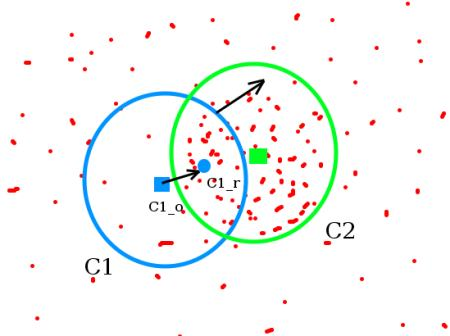
\includegraphics{meanshift_basics.jpg}

The initial window is shown in blue circle with the name ``C1''. Its
original center is marked in blue rectangle, named ``C1\_o''. But if you
find the centroid of the points inside that window, you will get the
point ``C1\_r'' (marked in small blue circle) which is the real centroid
of the window. Surely they don't match. So move your window such that
the circle of the new window matches with the previous centroid. Again
find the new centroid. Most probably, it won't match. So move it again,
and continue the iterations such that the center of window and its
centroid falls on the same location (or within a small desired error).
So finally what you obtain is a window with maximum pixel distribution.
It is marked with a green circle, named ``C2''. As you can see in the
image, it has maximum number of points. The whole process is
demonstrated on a static image below:
\includegraphics{meanshift_face.gif} So we normally pass the histogram
backprojected image and initial target location. When the object moves,
obviously the movement is reflected in the histogram backprojected
image. As a result, the meanshift algorithm moves our window to the new
location with maximum density.

    \hypertarget{an-actual-object-tracker-by-using-the-mean-shift}{%
\subsubsection{1.2 An actual object tracker by using the mean
shift}\label{an-actual-object-tracker-by-using-the-mean-shift}}

    \begin{Verbatim}[commandchars=\\\{\}]
{\color{incolor}In [{\color{incolor}3}]:} \PY{k+kn}{from} \PY{n+nn}{motion} \PY{k}{import} \PY{o}{*}
        \PY{k+kn}{import} \PY{n+nn}{cv2}
        \PY{n}{plt}\PY{o}{.}\PY{n}{rcParams}\PY{p}{[}\PY{l+s+s1}{\PYZsq{}}\PY{l+s+s1}{figure.figsize}\PY{l+s+s1}{\PYZsq{}}\PY{p}{]} \PY{o}{=} \PY{p}{(}\PY{l+m+mi}{20}\PY{p}{,} \PY{l+m+mi}{4}\PY{p}{)} \PY{c+c1}{\PYZsh{}set default size of plots}
        
        \PY{n}{path} \PY{o}{=} \PY{l+s+s2}{\PYZdq{}}\PY{l+s+s2}{BlurBody/img2/}\PY{l+s+s2}{\PYZdq{}}
        \PY{c+c1}{\PYZsh{}\PYZsh{} NEED TO ADD SORTED() HERE}
        \PY{n}{list\PYZus{}image} \PY{o}{=} \PY{p}{[}\PY{p}{]}
        \PY{n}{list\PYZus{}image} \PY{o}{=} \PY{n+nb}{sorted}\PY{p}{(}\PY{n}{listdir}\PY{p}{(}\PY{n}{path}\PY{p}{,}\PY{n}{list\PYZus{}image}\PY{p}{)}\PY{p}{)}
        \PY{n+nb}{print}\PY{p}{(}\PY{n+nb}{len}\PY{p}{(}\PY{n}{list\PYZus{}image}\PY{p}{)}\PY{p}{)}
        
        \PY{n}{frame1} \PY{o}{=} \PY{n}{cv2}\PY{o}{.}\PY{n}{imread}\PY{p}{(}\PY{n}{list\PYZus{}image}\PY{p}{[}\PY{l+m+mi}{0}\PY{p}{]}\PY{p}{)}
        \PY{n}{x}\PY{p}{,} \PY{n}{y}\PY{p}{,} \PY{n}{w}\PY{p}{,} \PY{n}{h} \PY{o}{=} \PY{l+m+mi}{400}\PY{p}{,}\PY{l+m+mi}{48}\PY{p}{,}\PY{l+m+mi}{87}\PY{p}{,}\PY{l+m+mi}{319} \PY{c+c1}{\PYZsh{} Blur body}
        \PY{n}{track\PYZus{}window} \PY{o}{=} \PY{p}{(}\PY{n}{x}\PY{p}{,}\PY{n}{y}\PY{p}{,}\PY{n}{w}\PY{p}{,}\PY{n}{h}\PY{p}{)}
        \PY{n}{roi} \PY{o}{=} \PY{n}{frame1}\PY{p}{[}\PY{n}{y}\PY{p}{:}\PY{n}{y}\PY{o}{+}\PY{n}{h}\PY{p}{,}\PY{n}{x}\PY{p}{:}\PY{n}{x}\PY{o}{+}\PY{n}{w}\PY{p}{]}
        
        \PY{n}{hsv\PYZus{}roi} \PY{o}{=} \PY{n}{cv2}\PY{o}{.}\PY{n}{cvtColor}\PY{p}{(}\PY{n}{roi}\PY{p}{,}\PY{n}{cv2}\PY{o}{.}\PY{n}{COLOR\PYZus{}BGR2HSV}\PY{p}{)}
        \PY{c+c1}{\PYZsh{}\PYZsh{}\PYZsh{}\PYZsh{}\PYZsh{}\PYZsh{}\PYZsh{}\PYZsh{}\PYZsh{}\PYZsh{}\PYZsh{}\PYZsh{}\PYZsh{}\PYZsh{}\PYZsh{}\PYZsh{}\PYZsh{}\PYZsh{}\PYZsh{}\PYZsh{}\PYZsh{}\PYZsh{}\PYZsh{}\PYZsh{}\PYZsh{}\PYZsh{}\PYZsh{}\PYZsh{}\PYZsh{}\PYZsh{}\PYZsh{}\PYZsh{}\PYZsh{}\PYZsh{}\PYZsh{}\PYZsh{}\PYZsh{}\PYZsh{}\PYZsh{}\PYZsh{}\PYZsh{}\PYZsh{}\PYZsh{}\PYZsh{}\PYZsh{}\PYZsh{}\PYZsh{}\PYZsh{}\PYZsh{}\PYZsh{}\PYZsh{}\PYZsh{}\PYZsh{}}
        \PY{c+c1}{\PYZsh{} You may modify the code below to use the params you}
        \PY{c+c1}{\PYZsh{} define above.}
        \PY{n}{thresh\PYZus{}value1} \PY{o}{=} \PY{l+m+mf}{60.}
        \PY{n}{thresh\PYZus{}value2} \PY{o}{=} \PY{l+m+mf}{20.}
        \PY{n}{channel} \PY{o}{=} \PY{l+m+mi}{1}
        \PY{c+c1}{\PYZsh{}\PYZsh{}\PYZsh{}\PYZsh{}\PYZsh{}\PYZsh{}\PYZsh{}\PYZsh{}\PYZsh{}\PYZsh{}\PYZsh{}\PYZsh{}\PYZsh{}\PYZsh{}\PYZsh{}\PYZsh{}\PYZsh{}\PYZsh{}\PYZsh{}\PYZsh{}\PYZsh{}\PYZsh{}\PYZsh{}\PYZsh{}\PYZsh{}\PYZsh{}\PYZsh{}\PYZsh{}\PYZsh{}\PYZsh{}\PYZsh{}\PYZsh{}\PYZsh{}\PYZsh{}\PYZsh{}\PYZsh{}\PYZsh{}\PYZsh{}\PYZsh{}\PYZsh{}\PYZsh{}\PYZsh{}\PYZsh{}\PYZsh{}\PYZsh{}\PYZsh{}\PYZsh{}\PYZsh{}\PYZsh{}\PYZsh{}\PYZsh{}\PYZsh{}\PYZsh{}}
        \PY{n}{mask} \PY{o}{=} \PY{n}{cv2}\PY{o}{.}\PY{n}{inRange}\PY{p}{(}\PY{n}{hsv\PYZus{}roi}\PY{p}{,}\PY{n}{np}\PY{o}{.}\PY{n}{array}\PY{p}{(}\PY{p}{(}\PY{l+m+mf}{0.}\PY{p}{,}\PY{n}{thresh\PYZus{}value1}\PY{p}{,}\PY{n}{thresh\PYZus{}value2}\PY{p}{,}\PY{p}{)}\PY{p}{)}\PY{p}{,}\PY{n}{np}\PY{o}{.}\PY{n}{array}\PY{p}{(}\PY{p}{(}\PY{l+m+mf}{180.}\PY{p}{,}\PY{l+m+mf}{255.}\PY{p}{,}\PY{l+m+mf}{255.}\PY{p}{,}\PY{p}{)}\PY{p}{)}\PY{p}{)} \PY{c+c1}{\PYZsh{} Blur body}
        \PY{n}{roi\PYZus{}hist} \PY{o}{=} \PY{n}{cv2}\PY{o}{.}\PY{n}{calcHist}\PY{p}{(}\PY{p}{[}\PY{n}{hsv\PYZus{}roi}\PY{p}{]}\PY{p}{,}\PY{p}{[}\PY{n}{channel}\PY{p}{]}\PY{p}{,}\PY{n}{mask}\PY{p}{,}\PY{p}{[}\PY{l+m+mi}{180}\PY{p}{]}\PY{p}{,}\PY{p}{[}\PY{l+m+mi}{0}\PY{p}{,}\PY{l+m+mi}{180}\PY{p}{]}\PY{p}{)}
        \PY{n}{roi\PYZus{}hist1} \PY{o}{=} \PY{n}{cv2}\PY{o}{.}\PY{n}{calcHist}\PY{p}{(}\PY{p}{[}\PY{n}{hsv\PYZus{}roi}\PY{p}{]}\PY{p}{,}\PY{p}{[}\PY{n}{channel}\PY{p}{]}\PY{p}{,}\PY{k+kc}{None}\PY{p}{,}\PY{p}{[}\PY{l+m+mi}{180}\PY{p}{]}\PY{p}{,}\PY{p}{[}\PY{l+m+mi}{0}\PY{p}{,}\PY{l+m+mi}{180}\PY{p}{]}\PY{p}{)}
        
        
        \PY{n}{plt}\PY{o}{.}\PY{n}{subplot}\PY{p}{(}\PY{l+m+mi}{1}\PY{p}{,}\PY{l+m+mi}{5}\PY{p}{,}\PY{l+m+mi}{1}\PY{p}{)}
        \PY{n}{plt}\PY{o}{.}\PY{n}{imshow}\PY{p}{(}\PY{n}{roi}\PY{p}{)}
        \PY{n}{plt}\PY{o}{.}\PY{n}{axis}\PY{p}{(}\PY{l+s+s1}{\PYZsq{}}\PY{l+s+s1}{off}\PY{l+s+s1}{\PYZsq{}}\PY{p}{)}
        \PY{n}{plt}\PY{o}{.}\PY{n}{title}\PY{p}{(}\PY{l+s+s1}{\PYZsq{}}\PY{l+s+s1}{roi\PYZus{}image}\PY{l+s+s1}{\PYZsq{}}\PY{p}{)}
        
        \PY{n}{plt}\PY{o}{.}\PY{n}{subplot}\PY{p}{(}\PY{l+m+mi}{1}\PY{p}{,}\PY{l+m+mi}{5}\PY{p}{,}\PY{l+m+mi}{2}\PY{p}{)}
        \PY{n}{plt}\PY{o}{.}\PY{n}{imshow}\PY{p}{(}\PY{n}{hsv\PYZus{}roi}\PY{p}{)}
        \PY{n}{plt}\PY{o}{.}\PY{n}{axis}\PY{p}{(}\PY{l+s+s1}{\PYZsq{}}\PY{l+s+s1}{off}\PY{l+s+s1}{\PYZsq{}}\PY{p}{)}
        \PY{n}{plt}\PY{o}{.}\PY{n}{title}\PY{p}{(}\PY{l+s+s1}{\PYZsq{}}\PY{l+s+s1}{Hsv\PYZus{}roi\PYZus{}image}\PY{l+s+s1}{\PYZsq{}}\PY{p}{)}
        
        \PY{n}{plt}\PY{o}{.}\PY{n}{subplot}\PY{p}{(}\PY{l+m+mi}{1}\PY{p}{,}\PY{l+m+mi}{5}\PY{p}{,}\PY{l+m+mi}{3}\PY{p}{)}
        \PY{n}{plt}\PY{o}{.}\PY{n}{imshow}\PY{p}{(}\PY{n}{mask}\PY{p}{)}
        \PY{n}{plt}\PY{o}{.}\PY{n}{axis}\PY{p}{(}\PY{l+s+s1}{\PYZsq{}}\PY{l+s+s1}{off}\PY{l+s+s1}{\PYZsq{}}\PY{p}{)}
        \PY{n}{plt}\PY{o}{.}\PY{n}{title}\PY{p}{(}\PY{l+s+s1}{\PYZsq{}}\PY{l+s+s1}{Mask\PYZus{}image}\PY{l+s+s1}{\PYZsq{}}\PY{p}{)}
        
        \PY{n}{plt}\PY{o}{.}\PY{n}{subplot}\PY{p}{(}\PY{l+m+mi}{1}\PY{p}{,}\PY{l+m+mi}{5}\PY{p}{,}\PY{l+m+mi}{4}\PY{p}{)}
        \PY{n}{y1} \PY{o}{=} \PY{n}{np}\PY{o}{.}\PY{n}{squeeze}\PY{p}{(}\PY{n}{roi\PYZus{}hist1}\PY{p}{)}
        \PY{n}{y1} \PY{o}{=}\PY{n+nb}{list}\PY{p}{(}\PY{n}{y1}\PY{p}{)}
        \PY{n}{x1} \PY{o}{=} \PY{n+nb}{list}\PY{p}{(}\PY{n+nb}{range}\PY{p}{(}\PY{l+m+mi}{1}\PY{p}{,}\PY{l+m+mi}{181}\PY{p}{,}\PY{l+m+mi}{1}\PY{p}{)}\PY{p}{)}
        \PY{n}{plt}\PY{o}{.}\PY{n}{title}\PY{p}{(}\PY{l+s+s2}{\PYZdq{}}\PY{l+s+s2}{Original\PYZus{}hist}\PY{l+s+s2}{\PYZdq{}}\PY{p}{)}
        \PY{n}{plt}\PY{o}{.}\PY{n}{bar}\PY{p}{(}\PY{n}{x1}\PY{p}{,}\PY{n}{y1}\PY{p}{)}
        
        \PY{n}{plt}\PY{o}{.}\PY{n}{subplot}\PY{p}{(}\PY{l+m+mi}{1}\PY{p}{,}\PY{l+m+mi}{5}\PY{p}{,}\PY{l+m+mi}{5}\PY{p}{)}
        \PY{n}{y1} \PY{o}{=} \PY{n}{np}\PY{o}{.}\PY{n}{squeeze}\PY{p}{(}\PY{n}{roi\PYZus{}hist}\PY{p}{)}
        \PY{n}{y1} \PY{o}{=}\PY{n+nb}{list}\PY{p}{(}\PY{n}{y1}\PY{p}{)}
        \PY{n}{x1} \PY{o}{=} \PY{n+nb}{list}\PY{p}{(}\PY{n+nb}{range}\PY{p}{(}\PY{l+m+mi}{1}\PY{p}{,}\PY{l+m+mi}{181}\PY{p}{,}\PY{l+m+mi}{1}\PY{p}{)}\PY{p}{)}
        \PY{n}{plt}\PY{o}{.}\PY{n}{title}\PY{p}{(}\PY{l+s+s2}{\PYZdq{}}\PY{l+s+s2}{mask\PYZus{}hist}\PY{l+s+s2}{\PYZdq{}}\PY{p}{)}
        \PY{n}{plt}\PY{o}{.}\PY{n}{bar}\PY{p}{(}\PY{n}{x1}\PY{p}{,}\PY{n}{y1}\PY{p}{)}
        \PY{n}{plt}\PY{o}{.}\PY{n}{show}\PY{p}{(}\PY{p}{)}
\end{Verbatim}


    \begin{Verbatim}[commandchars=\\\{\}]
334

    \end{Verbatim}

    \begin{center}
    \adjustimage{max size={0.9\linewidth}{0.9\paperheight}}{output_6_1.png}
    \end{center}
    { \hspace*{\fill} \\}
    
    \begin{Verbatim}[commandchars=\\\{\}]
{\color{incolor}In [{\color{incolor}4}]:} \PY{n}{frame1} \PY{o}{=} \PY{n}{cv2}\PY{o}{.}\PY{n}{imread}\PY{p}{(}\PY{n}{list\PYZus{}image}\PY{p}{[}\PY{l+m+mi}{0}\PY{p}{]}\PY{p}{)}
        \PY{n}{hsv\PYZus{}frame1} \PY{o}{=} \PY{n}{cv2}\PY{o}{.}\PY{n}{cvtColor}\PY{p}{(}\PY{n}{frame1}\PY{p}{,}\PY{n}{cv2}\PY{o}{.}\PY{n}{COLOR\PYZus{}BGR2HSV}\PY{p}{)}
        \PY{n}{dst} \PY{o}{=} \PY{n}{cv2}\PY{o}{.}\PY{n}{calcBackProject}\PY{p}{(}\PY{p}{[}\PY{n}{hsv\PYZus{}frame1}\PY{p}{]}\PY{p}{,}\PY{p}{[}\PY{n}{channel}\PY{p}{]}\PY{p}{,}\PY{n}{roi\PYZus{}hist}\PY{p}{,}\PY{p}{[}\PY{l+m+mi}{0}\PY{p}{,}\PY{l+m+mi}{180}\PY{p}{]}\PY{p}{,}\PY{l+m+mi}{1}\PY{p}{)}
        
        \PY{n}{plt}\PY{o}{.}\PY{n}{rcParams}\PY{p}{[}\PY{l+s+s1}{\PYZsq{}}\PY{l+s+s1}{figure.figsize}\PY{l+s+s1}{\PYZsq{}}\PY{p}{]} \PY{o}{=} \PY{p}{(}\PY{l+m+mi}{20}\PY{p}{,} \PY{l+m+mi}{10}\PY{p}{)}
        
        \PY{n}{plt}\PY{o}{.}\PY{n}{subplot}\PY{p}{(}\PY{l+m+mi}{1}\PY{p}{,}\PY{l+m+mi}{2}\PY{p}{,}\PY{l+m+mi}{1}\PY{p}{)}
        \PY{n}{plt}\PY{o}{.}\PY{n}{imshow}\PY{p}{(}\PY{n}{hsv\PYZus{}frame1}\PY{p}{)}
        \PY{n}{plt}\PY{o}{.}\PY{n}{axis}\PY{p}{(}\PY{l+s+s1}{\PYZsq{}}\PY{l+s+s1}{off}\PY{l+s+s1}{\PYZsq{}}\PY{p}{)}
        \PY{n}{plt}\PY{o}{.}\PY{n}{title}\PY{p}{(}\PY{l+s+s1}{\PYZsq{}}\PY{l+s+s1}{hsv\PYZus{}frame1}\PY{l+s+s1}{\PYZsq{}}\PY{p}{)}
        
        \PY{n}{plt}\PY{o}{.}\PY{n}{subplot}\PY{p}{(}\PY{l+m+mi}{1}\PY{p}{,}\PY{l+m+mi}{2}\PY{p}{,}\PY{l+m+mi}{2}\PY{p}{)}
        \PY{n}{plt}\PY{o}{.}\PY{n}{imshow}\PY{p}{(}\PY{n}{dst}\PY{p}{)}
        \PY{n}{plt}\PY{o}{.}\PY{n}{axis}\PY{p}{(}\PY{l+s+s1}{\PYZsq{}}\PY{l+s+s1}{off}\PY{l+s+s1}{\PYZsq{}}\PY{p}{)}
        \PY{n}{plt}\PY{o}{.}\PY{n}{title}\PY{p}{(}\PY{l+s+s1}{\PYZsq{}}\PY{l+s+s1}{BackProject}\PY{l+s+s1}{\PYZsq{}}\PY{p}{)}
        \PY{n}{plt}\PY{o}{.}\PY{n}{show}\PY{p}{(}\PY{p}{)}
\end{Verbatim}


    \begin{center}
    \adjustimage{max size={0.9\linewidth}{0.9\paperheight}}{output_7_0.png}
    \end{center}
    { \hspace*{\fill} \\}
    
    \begin{Verbatim}[commandchars=\\\{\}]
{\color{incolor}In [{\color{incolor} }]:} \PY{k+kn}{from} \PY{n+nn}{motion} \PY{k}{import} \PY{n}{meanShift}\PY{p}{,}\PY{n}{listdir}
        \PY{k+kn}{from} \PY{n+nn}{utils} \PY{k}{import} \PY{o}{*}
        \PY{c+c1}{\PYZsh{}import numpy as np }
        \PY{c+c1}{\PYZsh{} Initailze bounding box}
        \PY{n}{bboxes} \PY{o}{=} \PY{p}{[}\PY{p}{]}
        \PY{n}{path} \PY{o}{=} \PY{l+s+s2}{\PYZdq{}}\PY{l+s+s2}{BlurBody/img2/}\PY{l+s+s2}{\PYZdq{}}
        \PY{n}{x}\PY{p}{,} \PY{n}{y}\PY{p}{,} \PY{n}{w}\PY{p}{,} \PY{n}{h} \PY{o}{=} \PY{l+m+mi}{400}\PY{p}{,}\PY{l+m+mi}{48}\PY{p}{,}\PY{l+m+mi}{87}\PY{p}{,}\PY{l+m+mi}{319} \PY{c+c1}{\PYZsh{} Blur body}
        \PY{n}{track\PYZus{}window} \PY{o}{=} \PY{p}{(}\PY{n}{x}\PY{p}{,}\PY{n}{y}\PY{p}{,}\PY{n}{w}\PY{p}{,}\PY{n}{h}\PY{p}{)}
        \PY{n}{list\PYZus{}image} \PY{o}{=} \PY{p}{[}\PY{p}{]}
        \PY{c+c1}{\PYZsh{}\PYZsh{} AGAIN THE SORTED PROBLEM}
        \PY{n}{list\PYZus{}image} \PY{o}{=} \PY{n+nb}{sorted}\PY{p}{(}\PY{n}{listdir}\PY{p}{(}\PY{n}{path}\PY{p}{,}\PY{n}{list\PYZus{}image}\PY{p}{)}\PY{p}{)}
        \PY{n+nb}{print}\PY{p}{(}\PY{n+nb}{len}\PY{p}{(}\PY{n}{list\PYZus{}image}\PY{p}{)}\PY{p}{)} 
        
        \PY{c+c1}{\PYZsh{}dsts = []}
        \PY{k}{for} \PY{n}{i} \PY{o+ow}{in} \PY{n+nb}{range}\PY{p}{(}\PY{n+nb}{len}\PY{p}{(}\PY{n}{list\PYZus{}image}\PY{p}{)}\PY{p}{)}\PY{p}{:}
            \PY{n}{frame} \PY{o}{=} \PY{n}{cv2}\PY{o}{.}\PY{n}{imread}\PY{p}{(}\PY{n}{list\PYZus{}image}\PY{p}{[}\PY{n}{i}\PY{p}{]}\PY{p}{)}
            \PY{n}{hsv} \PY{o}{=} \PY{n}{cv2}\PY{o}{.}\PY{n}{cvtColor}\PY{p}{(}\PY{n}{frame}\PY{p}{,}\PY{n}{cv2}\PY{o}{.}\PY{n}{COLOR\PYZus{}BGR2HSV}\PY{p}{)}
            \PY{n}{dst} \PY{o}{=} \PY{n}{cv2}\PY{o}{.}\PY{n}{calcBackProject}\PY{p}{(}\PY{p}{[}\PY{n}{hsv}\PY{p}{]}\PY{p}{,}\PY{p}{[}\PY{n}{channel}\PY{p}{]}\PY{p}{,}\PY{n}{roi\PYZus{}hist}\PY{p}{,}\PY{p}{[}\PY{l+m+mi}{0}\PY{p}{,}\PY{l+m+mi}{180}\PY{p}{]}\PY{p}{,}\PY{l+m+mi}{1}\PY{p}{)}
            \PY{c+c1}{\PYZsh{}dsts.append(dst)}
            \PY{n}{c} \PY{o}{=} \PY{n}{np}\PY{o}{.}\PY{n}{reshape}\PY{p}{(}\PY{n}{dst}\PY{p}{,}\PY{p}{(}\PY{o}{\PYZhy{}}\PY{l+m+mi}{1}\PY{p}{,}\PY{l+m+mi}{1}\PY{p}{)}\PY{p}{)}
            
            \PY{c+c1}{\PYZsh{}aplly meanshift to get the new location}
            \PY{n}{track\PYZus{}window} \PY{o}{=} \PY{n}{meanShift}\PY{p}{(}\PY{n}{dst}\PY{p}{,}\PY{n}{track\PYZus{}window}\PY{p}{,}\PY{n}{max\PYZus{}iter}\PY{o}{=}\PY{l+m+mi}{10}\PY{p}{,}\PY{n}{stop\PYZus{}thresh}\PY{o}{=}\PY{l+m+mf}{0.1}\PY{p}{)}
            \PY{n}{x}\PY{p}{,}\PY{n}{y}\PY{p}{,}\PY{n}{w}\PY{p}{,}\PY{n}{h} \PY{o}{=} \PY{n}{track\PYZus{}window}
            \PY{n}{bboxes}\PY{o}{.}\PY{n}{append}\PY{p}{(}\PY{p}{(}\PY{n}{x}\PY{p}{,}\PY{n}{y}\PY{p}{,}\PY{n}{w}\PY{p}{,}\PY{n}{h}\PY{p}{)}\PY{p}{)}
        
        \PY{n}{ani} \PY{o}{=} \PY{n}{animated\PYZus{}bbox}\PY{p}{(}\PY{n}{frames}\PY{p}{,} \PY{n}{bboxes}\PY{p}{)}
        \PY{n}{HTML}\PY{p}{(}\PY{n}{ani}\PY{o}{.}\PY{n}{to\PYZus{}html5\PYZus{}video}\PY{p}{(}\PY{p}{)}\PY{p}{)}
\end{Verbatim}


    \begin{Verbatim}[commandchars=\\\{\}]
334
{\ldots}
    \end{Verbatim}

    \hypertarget{evaluating-object-tracker-intersection-over-union-iou}{%
\subsubsection{1.3 Evaluating Object Tracker: intersection over union
(IoU)}\label{evaluating-object-tracker-intersection-over-union-iou}}

Intersection over union is a common metric for evaluating performance of
an object tracker. Implement \texttt{IoU} in \texttt{motion.py} to
evaluate our object tracker. You will full marks for IoU score
\textgreater{} 0.65.

    \begin{Verbatim}[commandchars=\\\{\}]
{\color{incolor}In [{\color{incolor} }]:} \PY{k+kn}{from} \PY{n+nn}{motion} \PY{k}{import} \PY{n}{IoU}
        \PY{c+c1}{\PYZsh{}load the graound\PYZus{}truth }
        
        \PY{n}{ground\PYZus{}path} \PY{o}{=} \PY{l+s+s2}{\PYZdq{}}\PY{l+s+s2}{BlurBody/groundtruth\PYZus{}rect.txt}\PY{l+s+s2}{\PYZdq{}}
        \PY{n}{f} \PY{o}{=} \PY{n+nb}{open}\PY{p}{(}\PY{n}{ground\PYZus{}path}\PY{p}{)}
        \PY{n}{gt\PYZus{}bboxes} \PY{o}{=} \PY{p}{[}\PY{p}{]}
        \PY{n}{ground\PYZus{}truth} \PY{o}{=} \PY{n}{f}\PY{o}{.}\PY{n}{readlines}\PY{p}{(}\PY{p}{)}
        \PY{n+nb}{print}\PY{p}{(}\PY{n+nb}{len}\PY{p}{(}\PY{n}{ground\PYZus{}truth}\PY{p}{)}\PY{p}{)}
        \PY{k}{for} \PY{n}{i} \PY{o+ow}{in} \PY{n+nb}{range}\PY{p}{(}\PY{n+nb}{len}\PY{p}{(}\PY{n}{ground\PYZus{}truth}\PY{p}{)}\PY{p}{)}\PY{p}{:}
            \PY{n}{x} \PY{o}{=} \PY{n+nb}{int}\PY{p}{(}\PY{n}{ground\PYZus{}truth}\PY{p}{[}\PY{n}{i}\PY{p}{]}\PY{o}{.}\PY{n}{split}\PY{p}{(}\PY{p}{)}\PY{p}{[}\PY{l+m+mi}{0}\PY{p}{]}\PY{p}{)}
            \PY{n}{y} \PY{o}{=} \PY{n+nb}{int}\PY{p}{(}\PY{n}{ground\PYZus{}truth}\PY{p}{[}\PY{n}{i}\PY{p}{]}\PY{o}{.}\PY{n}{split}\PY{p}{(}\PY{p}{)}\PY{p}{[}\PY{l+m+mi}{1}\PY{p}{]}\PY{p}{)}
            \PY{n}{w} \PY{o}{=} \PY{n+nb}{int}\PY{p}{(}\PY{n}{ground\PYZus{}truth}\PY{p}{[}\PY{n}{i}\PY{p}{]}\PY{o}{.}\PY{n}{split}\PY{p}{(}\PY{p}{)}\PY{p}{[}\PY{l+m+mi}{2}\PY{p}{]}\PY{p}{)}
            \PY{n}{h} \PY{o}{=} \PY{n+nb}{int}\PY{p}{(}\PY{n}{ground\PYZus{}truth}\PY{p}{[}\PY{n}{i}\PY{p}{]}\PY{o}{.}\PY{n}{split}\PY{p}{(}\PY{p}{)}\PY{p}{[}\PY{l+m+mi}{3}\PY{p}{]}\PY{p}{)}
            \PY{n}{gt\PYZus{}bboxes}\PY{o}{.}\PY{n}{append}\PY{p}{(}\PY{p}{(}\PY{n}{x}\PY{p}{,}\PY{n}{y}\PY{p}{,}\PY{n}{w}\PY{p}{,}\PY{n}{h}\PY{p}{)}\PY{p}{)}
        \PY{c+c1}{\PYZsh{}calculate the IOU}
        \PY{n}{average\PYZus{}iou} \PY{o}{=} \PY{l+m+mf}{0.0}
        \PY{k}{for} \PY{n}{gt\PYZus{}bbox}\PY{p}{,} \PY{n}{bbox} \PY{o+ow}{in} \PY{n+nb}{zip}\PY{p}{(}\PY{n}{gt\PYZus{}bboxes}\PY{p}{,} \PY{n}{bboxes}\PY{p}{)}\PY{p}{:}
            \PY{n}{average\PYZus{}iou} \PY{o}{+}\PY{o}{=} \PY{n}{IoU}\PY{p}{(}\PY{n}{gt\PYZus{}bbox}\PY{p}{,} \PY{n}{bbox}\PY{p}{)}
            \PY{c+c1}{\PYZsh{}print(IoU(gt\PYZus{}bbox, bbox))}
            
        \PY{n}{average\PYZus{}iou} \PY{o}{/}\PY{o}{=} \PY{n+nb}{len}\PY{p}{(}\PY{n}{gt\PYZus{}bboxes}\PY{p}{)}
        \PY{n+nb}{print}\PY{p}{(}\PY{n}{average\PYZus{}iou}\PY{p}{)}
\end{Verbatim}


    \hypertarget{lucas-kanade-method-for-optical-flow}{%
\subsection{2. Lucas-Kanade Method for Optical
Flow}\label{lucas-kanade-method-for-optical-flow}}

\hypertarget{deriving-optical-flow-equation}{%
\subsubsection{2.1 Deriving optical flow
equation}\label{deriving-optical-flow-equation}}

Optical flow methods are used to estimate motion of objects between two
consecutive image frames. For example, in the video below, the can of
tea seems to be moving to the left. For our system to be able to
understand that the can is moving to the left, it would be useful to
find a way to add vectors to the can (known as \textbf{flow vectors})
which point to the left, thus describing its motion.

Given two consecutive frames, how can we find the flow vectors for the
first frame which describe how objects move between frames? To start, we
make a reasonable assumption called the \textbf{brightness constancy}
assumption: the pixel intensity of a moving point stays the same between
two consecutive frames with small time difference. In other words,
picking any pixel of the moving can, its brightness stays approximately
the same between frames--its movement should not affect its brightness
after all.

Consider pixel intensity (a.k.a. brightness) \(I(x, y, t)\) of a point
\((x, y)\) in the first frame \(t\). Suppose that the point has moved to
\((x+\Delta{x}, y+\Delta{y})\) after \(\Delta{t}\). According to the
brightness constancy assumption, we can relate intensities of the point
in the two frames using the following equation:

\[
I(x,y,t)=I(x+\Delta{x},y+\Delta{y},t+\Delta{t})
\]

Coming back to the example of the moving can, this equation simply
states that the point that we picked will have the same intensity even
after it moves in space \((\Delta{x}\) and \(\Delta{y})\) and between
frames \((\Delta{t})\). From this simple assumption, we can derive what
is known as the \textbf{optical flow equation}. For a given point for
any frame, the optical flow equation is given by:

\[
I_x({\mathbf{p}})v_{x} +
I_y({\mathbf{p}})v_{y} +
I_t({\mathbf{p}})
= 0
\]

Here, \(I_x\), \(I_y\) and \(I_t\) are partial derivatives of pixel
intensity \(I\). Meanwhile, \(v_{x}\) and \(v_{y}\) are \textbf{flow
vectors} in the \(x-\) and \(y-\)direction, respectively. These are the
vectors we care about! If we can solve for these two values, we will be
able to describe the motion of any object between frames.

    \begin{Verbatim}[commandchars=\\\{\}]
{\color{incolor}In [{\color{incolor}7}]:} \PY{c+c1}{\PYZsh{} Load frames}
        \PY{n}{frames} \PY{o}{=} \PY{n}{load\PYZus{}frames}\PY{p}{(}\PY{l+s+s2}{\PYZdq{}}\PY{l+s+s2}{images2/}\PY{l+s+s2}{\PYZdq{}}\PY{p}{)}
        \PY{n}{ani} \PY{o}{=} \PY{n}{animated\PYZus{}frames}\PY{p}{(}\PY{n}{frames}\PY{p}{)}
        \PY{n}{HTML}\PY{p}{(}\PY{n}{ani}\PY{o}{.}\PY{n}{to\PYZus{}html5\PYZus{}video}\PY{p}{(}\PY{p}{)}\PY{p}{)}
\end{Verbatim}


    \begin{Verbatim}[commandchars=\\\{\}]
/Users/databook/miniconda3/envs/cs4243/lib/python3.7/site-packages/skimage/io/\_io.py:48: UserWarning: `as\_grey` has been deprecated in favor of `as\_gray`
  warn('`as\_grey` has been deprecated in favor of `as\_gray`')

    \end{Verbatim}

\begin{Verbatim}[commandchars=\\\{\}]
{\color{outcolor}Out[{\color{outcolor}7}]:} <IPython.core.display.HTML object>
\end{Verbatim}
            
    \begin{center}
    \adjustimage{max size={0.9\linewidth}{0.9\paperheight}}{output_12_2.png}
    \end{center}
    { \hspace*{\fill} \\}
    
    \hypertarget{overview-of-lucas-kanade-method}{%
\subsubsection{2.2 Overview of Lucas-Kanade
method}\label{overview-of-lucas-kanade-method}}

One issue with the optical flow equation is that there are two unknowns
that we want to solve for (\(v_x\) and \(v_y\)). This problem is known
as the \textbf{aperture problem}. In other words, just looking an
``aperture'' at one pixel at a time, it is impossible to discern the
true direction of motion of the object in question.

The Lucas--Kanade method solves this problem by adding another
assumption: \textbf{spatial coherence}. That is, that the motion of the
image contents between two frames is approximately constant within a
neighborhood of the point \(p\) under consideration.

Consider a neighborhood of \(p\), \(N(p)=\{p_1,...,p_n\}\) (e.g.~3x3
window around \(p\)). Adding the spatial coherence assumption to the
optical flow equation, we see that the following should be satisfied:

For every \(p_i \in N(p)\), \[
I_{x}(p_i)v_x + I_{y}(p_i)v_y = -I_{t}(p_i)
\]

These equations can be written in matrix form \(Av=b\), where

\[
A = 
\begin{bmatrix}
    I_{x}(p_1) & I_{y}(p_1)\\
    I_{x}(p_2) & I_{y}(p_2)\\
    \vdots & \vdots\\
    I_{x}(p_n) & I_{y}(p_n)
\end{bmatrix}
\quad
v =
\begin{bmatrix}
    v_{x}\\
    v_{y}
\end{bmatrix}
\quad
b =
\begin{bmatrix}
    -I_{t}(p_1)\\
    -I_{t}(p_2)\\
    \vdots\\
    -I_{t}(p_n)
\end{bmatrix}
\]

We can now solve for the flow vectors (now represented as \(v\)) by
solving the following least-squares problem: \(A^{T}Av=A^{T}b\).

    \hypertarget{implementation-of-lucas-kanade-method}{%
\subsubsection{2.3 Implementation of Lucas-Kanade
method}\label{implementation-of-lucas-kanade-method}}

In this section, we are going to implement basic Lucas-Kanade method for
feature tracking. In order to do so, we first need to find keypoints to
track. Harris corner detector is commonly used to initialize the
keypoints to track with Lucas-Kanade method. For this assignment, we are
going to use
\href{http://scikit-image.org/docs/dev/auto_examples/features_detection/plot_corner.html}{\texttt{skimage}
implementation} of Harris corner detector.

    \begin{Verbatim}[commandchars=\\\{\}]
{\color{incolor}In [{\color{incolor}22}]:} \PY{k+kn}{from} \PY{n+nn}{skimage} \PY{k}{import} \PY{n}{filters}
         \PY{k+kn}{from} \PY{n+nn}{skimage}\PY{n+nn}{.}\PY{n+nn}{feature} \PY{k}{import} \PY{n}{corner\PYZus{}harris}\PY{p}{,} \PY{n}{corner\PYZus{}peaks}
         
         \PY{n}{frames} \PY{o}{=} \PY{n}{load\PYZus{}frames}\PY{p}{(}\PY{l+s+s1}{\PYZsq{}}\PY{l+s+s1}{images2}\PY{l+s+s1}{\PYZsq{}}\PY{p}{)}
         \PY{n+nb}{print}\PY{p}{(}\PY{n+nb}{len}\PY{p}{(}\PY{n}{frames}\PY{p}{)}\PY{p}{)}
         \PY{n+nb}{print}\PY{p}{(}\PY{n}{frames}\PY{p}{[}\PY{l+m+mi}{0}\PY{p}{]}\PY{o}{.}\PY{n}{shape}\PY{p}{)}
         
         \PY{c+c1}{\PYZsh{} Detect keypoints to track}
         \PY{n}{keypoints} \PY{o}{=} \PY{n}{corner\PYZus{}peaks}\PY{p}{(}\PY{n}{corner\PYZus{}harris}\PY{p}{(}\PY{n}{frames}\PY{p}{[}\PY{l+m+mi}{0}\PY{p}{]}\PY{p}{)}\PY{p}{,}
                                  \PY{n}{exclude\PYZus{}border}\PY{o}{=}\PY{l+m+mi}{5}\PY{p}{,}
                                  \PY{n}{threshold\PYZus{}rel}\PY{o}{=}\PY{l+m+mf}{0.01}\PY{p}{)}
         
         \PY{c+c1}{\PYZsh{} Plot kepoints}
         \PY{n}{plt}\PY{o}{.}\PY{n}{figure}\PY{p}{(}\PY{n}{figsize}\PY{o}{=}\PY{p}{(}\PY{l+m+mi}{15}\PY{p}{,}\PY{l+m+mi}{12}\PY{p}{)}\PY{p}{)}
         \PY{n}{plt}\PY{o}{.}\PY{n}{imshow}\PY{p}{(}\PY{n}{frames}\PY{p}{[}\PY{l+m+mi}{0}\PY{p}{]}\PY{p}{)}
         \PY{n}{plt}\PY{o}{.}\PY{n}{scatter}\PY{p}{(}\PY{n}{keypoints}\PY{p}{[}\PY{p}{:}\PY{p}{,}\PY{l+m+mi}{1}\PY{p}{]}\PY{p}{,} \PY{n}{keypoints}\PY{p}{[}\PY{p}{:}\PY{p}{,}\PY{l+m+mi}{0}\PY{p}{]}\PY{p}{,}
                     \PY{n}{facecolors}\PY{o}{=}\PY{l+s+s1}{\PYZsq{}}\PY{l+s+s1}{none}\PY{l+s+s1}{\PYZsq{}}\PY{p}{,} \PY{n}{edgecolors}\PY{o}{=}\PY{l+s+s1}{\PYZsq{}}\PY{l+s+s1}{r}\PY{l+s+s1}{\PYZsq{}}\PY{p}{)}
         \PY{n}{plt}\PY{o}{.}\PY{n}{axis}\PY{p}{(}\PY{l+s+s1}{\PYZsq{}}\PY{l+s+s1}{off}\PY{l+s+s1}{\PYZsq{}}\PY{p}{)}
         \PY{n}{plt}\PY{o}{.}\PY{n}{title}\PY{p}{(}\PY{l+s+s1}{\PYZsq{}}\PY{l+s+s1}{Detected keypoints in the first frame}\PY{l+s+s1}{\PYZsq{}}\PY{p}{)}
         \PY{n}{plt}\PY{o}{.}\PY{n}{show}\PY{p}{(}\PY{p}{)}
\end{Verbatim}


    \begin{Verbatim}[commandchars=\\\{\}]
/Users/databook/miniconda3/envs/cs4243/lib/python3.7/site-packages/skimage/io/\_io.py:48: UserWarning: `as\_grey` has been deprecated in favor of `as\_gray`
  warn('`as\_grey` has been deprecated in favor of `as\_gray`')

    \end{Verbatim}

    \begin{Verbatim}[commandchars=\\\{\}]
13
(494, 685)

    \end{Verbatim}

    \begin{center}
    \adjustimage{max size={0.9\linewidth}{0.9\paperheight}}{output_15_2.png}
    \end{center}
    { \hspace*{\fill} \\}
    
    Implement function \textbf{\texttt{lucas\_kanade}} in \texttt{motion.py}
and run the code cell below. You will be able to see small arrows
pointing towards the directions where keypoints are moving.

    \begin{Verbatim}[commandchars=\\\{\}]
{\color{incolor}In [{\color{incolor}28}]:} \PY{k+kn}{from} \PY{n+nn}{motion} \PY{k}{import} \PY{n}{lucas\PYZus{}kanade}
         
         \PY{c+c1}{\PYZsh{} Lucas\PYZhy{}Kanade method for optical flow}
         \PY{n}{flow\PYZus{}vectors} \PY{o}{=} \PY{n}{lucas\PYZus{}kanade}\PY{p}{(}\PY{n}{frames}\PY{p}{[}\PY{l+m+mi}{0}\PY{p}{]}\PY{p}{,} \PY{n}{frames}\PY{p}{[}\PY{l+m+mi}{1}\PY{p}{]}\PY{p}{,} \PY{n}{keypoints}\PY{p}{,} \PY{n}{window\PYZus{}size}\PY{o}{=}\PY{l+m+mi}{5}\PY{p}{)}
         
         \PY{c+c1}{\PYZsh{} Plot flow vectors}
         \PY{n}{plt}\PY{o}{.}\PY{n}{figure}\PY{p}{(}\PY{n}{figsize}\PY{o}{=}\PY{p}{(}\PY{l+m+mi}{15}\PY{p}{,}\PY{l+m+mi}{12}\PY{p}{)}\PY{p}{)}
         \PY{n}{plt}\PY{o}{.}\PY{n}{imshow}\PY{p}{(}\PY{n}{frames}\PY{p}{[}\PY{l+m+mi}{0}\PY{p}{]}\PY{p}{)}
         \PY{n}{plt}\PY{o}{.}\PY{n}{axis}\PY{p}{(}\PY{l+s+s1}{\PYZsq{}}\PY{l+s+s1}{off}\PY{l+s+s1}{\PYZsq{}}\PY{p}{)}
         \PY{n}{plt}\PY{o}{.}\PY{n}{title}\PY{p}{(}\PY{l+s+s1}{\PYZsq{}}\PY{l+s+s1}{Optical flow vectors}\PY{l+s+s1}{\PYZsq{}}\PY{p}{)}
         
         \PY{n+nb}{print}\PY{p}{(}\PY{n}{keypoints}\PY{o}{.}\PY{n}{shape}\PY{p}{,}\PY{n}{flow\PYZus{}vectors}\PY{o}{.}\PY{n}{shape}\PY{p}{)}
         \PY{k}{for} \PY{n}{y}\PY{p}{,} \PY{n}{x}\PY{p}{,} \PY{n}{vy}\PY{p}{,} \PY{n}{vx} \PY{o+ow}{in} \PY{n}{np}\PY{o}{.}\PY{n}{hstack}\PY{p}{(}\PY{p}{(}\PY{n}{keypoints}\PY{p}{,} \PY{n}{flow\PYZus{}vectors}\PY{p}{)}\PY{p}{)}\PY{p}{:}
             \PY{n}{plt}\PY{o}{.}\PY{n}{arrow}\PY{p}{(}\PY{n}{x}\PY{p}{,} \PY{n}{y}\PY{p}{,} \PY{n}{vx}\PY{p}{,} \PY{n}{vy}\PY{p}{,} \PY{n}{head\PYZus{}width}\PY{o}{=}\PY{l+m+mi}{5}\PY{p}{,} \PY{n}{head\PYZus{}length}\PY{o}{=}\PY{l+m+mi}{5}\PY{p}{,} \PY{n}{color}\PY{o}{=}\PY{l+s+s1}{\PYZsq{}}\PY{l+s+s1}{b}\PY{l+s+s1}{\PYZsq{}}\PY{p}{)}
             
\end{Verbatim}


    \begin{Verbatim}[commandchars=\\\{\}]
(295, 2) (295, 2)

    \end{Verbatim}

    \begin{center}
    \adjustimage{max size={0.9\linewidth}{0.9\paperheight}}{output_17_1.png}
    \end{center}
    { \hspace*{\fill} \\}
    
    We can estimate the position of the keypoints in the next frame by
adding the flow vectors to the keypoints.

    \begin{Verbatim}[commandchars=\\\{\}]
{\color{incolor}In [{\color{incolor}29}]:} \PY{c+c1}{\PYZsh{} Plot tracked kepoints}
         \PY{n}{new\PYZus{}keypoints} \PY{o}{=} \PY{n}{keypoints} \PY{o}{+} \PY{n}{flow\PYZus{}vectors}
         \PY{n}{plt}\PY{o}{.}\PY{n}{figure}\PY{p}{(}\PY{n}{figsize}\PY{o}{=}\PY{p}{(}\PY{l+m+mi}{15}\PY{p}{,}\PY{l+m+mi}{12}\PY{p}{)}\PY{p}{)}
         \PY{n}{plt}\PY{o}{.}\PY{n}{imshow}\PY{p}{(}\PY{n}{frames}\PY{p}{[}\PY{l+m+mi}{1}\PY{p}{]}\PY{p}{)}
         \PY{n}{plt}\PY{o}{.}\PY{n}{scatter}\PY{p}{(}\PY{n}{new\PYZus{}keypoints}\PY{p}{[}\PY{p}{:}\PY{p}{,}\PY{l+m+mi}{1}\PY{p}{]}\PY{p}{,} \PY{n}{new\PYZus{}keypoints}\PY{p}{[}\PY{p}{:}\PY{p}{,}\PY{l+m+mi}{0}\PY{p}{]}\PY{p}{,}
                     \PY{n}{facecolors}\PY{o}{=}\PY{l+s+s1}{\PYZsq{}}\PY{l+s+s1}{none}\PY{l+s+s1}{\PYZsq{}}\PY{p}{,} \PY{n}{edgecolors}\PY{o}{=}\PY{l+s+s1}{\PYZsq{}}\PY{l+s+s1}{r}\PY{l+s+s1}{\PYZsq{}}\PY{p}{)}
         \PY{n}{plt}\PY{o}{.}\PY{n}{axis}\PY{p}{(}\PY{l+s+s1}{\PYZsq{}}\PY{l+s+s1}{off}\PY{l+s+s1}{\PYZsq{}}\PY{p}{)}
         \PY{n}{plt}\PY{o}{.}\PY{n}{title}\PY{p}{(}\PY{l+s+s1}{\PYZsq{}}\PY{l+s+s1}{Tracked keypoints in the second frame}\PY{l+s+s1}{\PYZsq{}}\PY{p}{)}
         \PY{n}{plt}\PY{o}{.}\PY{n}{show}\PY{p}{(}\PY{p}{)}
\end{Verbatim}


    \begin{center}
    \adjustimage{max size={0.9\linewidth}{0.9\paperheight}}{output_19_0.png}
    \end{center}
    { \hspace*{\fill} \\}
    
    \hypertarget{feature-tracking-in-multiple-frames}{%
\subsubsection{2.4 Feature Tracking in multiple
frames}\label{feature-tracking-in-multiple-frames}}

Now we can use Lucas-Kanade method to track keypoints across multiple
frames. The idea is simple: compute flow vectors at keypoints in
\(i\)-th frame, and add the flow vectors to the points to keep track of
the points in \(i+1\)-th frame. We have provided the function
\texttt{track\_features} for you. First, run the code cell below. You
will notice that some of the points just drift away and are not tracked
very well.

Instead of keeping these `bad' tracks, we would want to somehow declare
some points are `lost' and just discard them. One simple way to is to
compare the patches around tracked points in two subsequent frames. If
the patch around a point is NOT similar to the patch around the
corresponding point in the next frame, then we declare the point to be
lost. Here, we are going to use mean squared error between two
normalized patches as the criterion for lost tracks.

Implement \textbf{\texttt{compute\_error}} in \texttt{motion.py}, and
re-run the code cell below. You will see many of the points disappearing
in later frames.

    \begin{Verbatim}[commandchars=\\\{\}]
{\color{incolor}In [{\color{incolor}30}]:} \PY{k+kn}{from} \PY{n+nn}{utils} \PY{k}{import} \PY{n}{animated\PYZus{}scatter}
         \PY{k+kn}{from} \PY{n+nn}{motion} \PY{k}{import} \PY{n}{track\PYZus{}features}
         \PY{c+c1}{\PYZsh{} Detect keypoints to track in the first frame}
         \PY{n}{keypoints} \PY{o}{=} \PY{n}{corner\PYZus{}peaks}\PY{p}{(}\PY{n}{corner\PYZus{}harris}\PY{p}{(}\PY{n}{frames}\PY{p}{[}\PY{l+m+mi}{0}\PY{p}{]}\PY{p}{)}\PY{p}{,}
                                  \PY{n}{exclude\PYZus{}border}\PY{o}{=}\PY{l+m+mi}{5}\PY{p}{,}
                                  \PY{n}{threshold\PYZus{}rel}\PY{o}{=}\PY{l+m+mf}{0.01}\PY{p}{)}
         
         \PY{n}{trajs} \PY{o}{=} \PY{n}{track\PYZus{}features}\PY{p}{(}\PY{n}{frames}\PY{p}{,} \PY{n}{keypoints}\PY{p}{,}
                                \PY{n}{error\PYZus{}thresh}\PY{o}{=}\PY{l+m+mf}{1.5}\PY{p}{,}
                                \PY{n}{optflow\PYZus{}fn}\PY{o}{=}\PY{n}{lucas\PYZus{}kanade}\PY{p}{,}
                                \PY{n}{window\PYZus{}size}\PY{o}{=}\PY{l+m+mi}{5}\PY{p}{)}
         \PY{n}{ani} \PY{o}{=} \PY{n}{animated\PYZus{}scatter}\PY{p}{(}\PY{n}{frames}\PY{p}{,}\PY{n}{trajs}\PY{p}{)}
         \PY{c+c1}{\PYZsh{}ani.save(\PYZdq{}images2.mp4\PYZdq{})}
         \PY{n}{HTML}\PY{p}{(}\PY{n}{ani}\PY{o}{.}\PY{n}{to\PYZus{}html5\PYZus{}video}\PY{p}{(}\PY{p}{)}\PY{p}{)}
\end{Verbatim}


\begin{Verbatim}[commandchars=\\\{\}]
{\color{outcolor}Out[{\color{outcolor}30}]:} <IPython.core.display.HTML object>
\end{Verbatim}
            
    \begin{center}
    \adjustimage{max size={0.9\linewidth}{0.9\paperheight}}{output_21_1.png}
    \end{center}
    { \hspace*{\fill} \\}
    
    \hypertarget{pyramidal-lucas-kanade-feature-tracker}{%
\subsection{3. Pyramidal Lucas-Kanade Feature
Tracker}\label{pyramidal-lucas-kanade-feature-tracker}}

In this section, we are going to implement a simpler version of the
method described in
\href{http://citeseerx.ist.psu.edu/viewdoc/download?doi=10.1.1.185.585\&rep=rep1\&type=pdf}{``Pyramidal
Implementation of the Lucas Kanade Feature Tracker''}.

    \hypertarget{iterative-lucas-kanade-method}{%
\subsubsection{3.1 Iterative Lucas-Kanade
method}\label{iterative-lucas-kanade-method}}

One limitation of the naive Lucas-Kanade method is that it cannot track
large motions between frames. You might have noticed that the resulting
flow vectors (blue arrows) in the previous section are too small that
the tracked keypoints are slightly off from where they should be. In
order to address this problem, we can iteratively refine the estimated
optical flow vectors. Below is the step-by-step description of the
algorithm:

Let \(p=\begin{bmatrix}p_x & p_y \end{bmatrix}^T\) be a point on frame
\(I\). The goal is to find flow vector
\(v=\begin{bmatrix}v_x & v_y \end{bmatrix}^T\) such that \(p+v\) is the
corresponding point of \(p\) on the next frame \(J\).

\begin{itemize}
\item
  Initialize flow vector: \[
  v=
  \begin{bmatrix}
    0\\0
  \end{bmatrix}
  \]
\item
  Compute spatial gradient matrix: \[
  G=\sum_{x=p_x-w}^{p_x+w}\sum_{y=p_y-w}^{p_y+w}
  \begin{bmatrix}
    I_{x}^2(x,y) & I_{x}(x,y)I_{y}(x,y)\\
    I_{x}(x,y)I_{y}(x,y) & I_{y}^2(x,y)
  \end{bmatrix}
  \]
\item
  \textbf{for \(k=1\) to \(K\)}

  \begin{itemize}
  \tightlist
  \item
    Compute temporal difference:
    \(\delta I_k(x, y) = I(x,y)-J(x+g_x+v_x, y+g_y+v_y)\)
  \item
    Compute image mismatch vector: \[
    b_k=\sum_{x=p_x-w}^{p_x+w}\sum_{y=p_y-w}^{p_y+w}
    \begin{bmatrix}
      \delta I_k(x, y)I_x(x,y)\\
      \delta I_k(x, y)I_y(x,y)
    \end{bmatrix}
    \]
  \item
    Compute optical flow: \(v^k=G^{-1}b_k\)
  \item
    Update flow vector for next iteration: \(v := v + v^k\)
  \end{itemize}
\item
  Return \(v\)
\end{itemize}

Implement \texttt{iterative\_lucas\_kanade} method in \texttt{motion.py}
and run the code cell below. You should be able to see slightly longer
arrows in the visualization.

    \begin{Verbatim}[commandchars=\\\{\}]
{\color{incolor}In [{\color{incolor}51}]:} \PY{k+kn}{from} \PY{n+nn}{motion} \PY{k}{import} \PY{n}{iterative\PYZus{}lucas\PYZus{}kanade}
         
         \PY{c+c1}{\PYZsh{} Run iterative Lucas\PYZhy{}Kanade method}
         \PY{n}{flow\PYZus{}vectors} \PY{o}{=} \PY{n}{iterative\PYZus{}lucas\PYZus{}kanade}\PY{p}{(}\PY{n}{frames}\PY{p}{[}\PY{l+m+mi}{0}\PY{p}{]}\PY{p}{,} \PY{n}{frames}\PY{p}{[}\PY{l+m+mi}{1}\PY{p}{]}\PY{p}{,} \PY{n}{keypoints}\PY{p}{)}
         
         \PY{c+c1}{\PYZsh{} Plot flow vectors}
         \PY{n}{plt}\PY{o}{.}\PY{n}{figure}\PY{p}{(}\PY{n}{figsize}\PY{o}{=}\PY{p}{(}\PY{l+m+mi}{15}\PY{p}{,}\PY{l+m+mi}{12}\PY{p}{)}\PY{p}{)}
         \PY{n}{plt}\PY{o}{.}\PY{n}{imshow}\PY{p}{(}\PY{n}{frames}\PY{p}{[}\PY{l+m+mi}{0}\PY{p}{]}\PY{p}{)}
         \PY{n}{plt}\PY{o}{.}\PY{n}{axis}\PY{p}{(}\PY{l+s+s1}{\PYZsq{}}\PY{l+s+s1}{off}\PY{l+s+s1}{\PYZsq{}}\PY{p}{)}
         \PY{n}{plt}\PY{o}{.}\PY{n}{title}\PY{p}{(}\PY{l+s+s1}{\PYZsq{}}\PY{l+s+s1}{Optical flow vectors (iterative LK)}\PY{l+s+s1}{\PYZsq{}}\PY{p}{)}
         
         \PY{k}{for} \PY{n}{y}\PY{p}{,} \PY{n}{x}\PY{p}{,} \PY{n}{vy}\PY{p}{,} \PY{n}{vx} \PY{o+ow}{in} \PY{n}{np}\PY{o}{.}\PY{n}{hstack}\PY{p}{(}\PY{p}{(}\PY{n}{keypoints}\PY{p}{,} \PY{n}{flow\PYZus{}vectors}\PY{p}{)}\PY{p}{)}\PY{p}{:}
             \PY{n}{plt}\PY{o}{.}\PY{n}{arrow}\PY{p}{(}\PY{n}{x}\PY{p}{,} \PY{n}{y}\PY{p}{,} \PY{n}{vx}\PY{p}{,} \PY{n}{vy}\PY{p}{,} \PY{n}{head\PYZus{}width}\PY{o}{=}\PY{l+m+mi}{5}\PY{p}{,} \PY{n}{head\PYZus{}length}\PY{o}{=}\PY{l+m+mi}{5}\PY{p}{,} \PY{n}{color}\PY{o}{=}\PY{l+s+s1}{\PYZsq{}}\PY{l+s+s1}{b}\PY{l+s+s1}{\PYZsq{}}\PY{p}{)}
\end{Verbatim}


    \begin{Verbatim}[commandchars=\\\{\}]
index out of bounds

    \end{Verbatim}

    \begin{center}
    \adjustimage{max size={0.9\linewidth}{0.9\paperheight}}{output_24_1.png}
    \end{center}
    { \hspace*{\fill} \\}
    
    \begin{Verbatim}[commandchars=\\\{\}]
{\color{incolor}In [{\color{incolor}52}]:} \PY{c+c1}{\PYZsh{} Plot tracked kepoints}
         \PY{n}{new\PYZus{}keypoints} \PY{o}{=} \PY{n}{keypoints} \PY{o}{+} \PY{n}{flow\PYZus{}vectors}
         \PY{n}{plt}\PY{o}{.}\PY{n}{figure}\PY{p}{(}\PY{n}{figsize}\PY{o}{=}\PY{p}{(}\PY{l+m+mi}{15}\PY{p}{,}\PY{l+m+mi}{12}\PY{p}{)}\PY{p}{)}
         \PY{n}{plt}\PY{o}{.}\PY{n}{imshow}\PY{p}{(}\PY{n}{frames}\PY{p}{[}\PY{l+m+mi}{1}\PY{p}{]}\PY{p}{)}
         \PY{n}{plt}\PY{o}{.}\PY{n}{scatter}\PY{p}{(}\PY{n}{new\PYZus{}keypoints}\PY{p}{[}\PY{p}{:}\PY{p}{,}\PY{l+m+mi}{1}\PY{p}{]}\PY{p}{,} \PY{n}{new\PYZus{}keypoints}\PY{p}{[}\PY{p}{:}\PY{p}{,}\PY{l+m+mi}{0}\PY{p}{]}\PY{p}{,}
                     \PY{n}{facecolors}\PY{o}{=}\PY{l+s+s1}{\PYZsq{}}\PY{l+s+s1}{none}\PY{l+s+s1}{\PYZsq{}}\PY{p}{,} \PY{n}{edgecolors}\PY{o}{=}\PY{l+s+s1}{\PYZsq{}}\PY{l+s+s1}{r}\PY{l+s+s1}{\PYZsq{}}\PY{p}{)}
         \PY{n}{plt}\PY{o}{.}\PY{n}{axis}\PY{p}{(}\PY{l+s+s1}{\PYZsq{}}\PY{l+s+s1}{off}\PY{l+s+s1}{\PYZsq{}}\PY{p}{)}
         \PY{n}{plt}\PY{o}{.}\PY{n}{title}\PY{p}{(}\PY{l+s+s1}{\PYZsq{}}\PY{l+s+s1}{Tracked keypoints in the second frame (iterative LK)}\PY{l+s+s1}{\PYZsq{}}\PY{p}{)}
         \PY{n}{plt}\PY{o}{.}\PY{n}{show}\PY{p}{(}\PY{p}{)}
\end{Verbatim}


    \begin{center}
    \adjustimage{max size={0.9\linewidth}{0.9\paperheight}}{output_25_0.png}
    \end{center}
    { \hspace*{\fill} \\}
    
    \begin{Verbatim}[commandchars=\\\{\}]
{\color{incolor}In [{\color{incolor}54}]:} \PY{c+c1}{\PYZsh{} Detect keypoints to track in the first frame}
         \PY{n}{keypoints} \PY{o}{=} \PY{n}{corner\PYZus{}peaks}\PY{p}{(}\PY{n}{corner\PYZus{}harris}\PY{p}{(}\PY{n}{frames}\PY{p}{[}\PY{l+m+mi}{0}\PY{p}{]}\PY{p}{)}\PY{p}{,}
                                  \PY{n}{exclude\PYZus{}border}\PY{o}{=}\PY{l+m+mi}{5}\PY{p}{,}
                                  \PY{n}{threshold\PYZus{}rel}\PY{o}{=}\PY{l+m+mf}{0.01}\PY{p}{)}
         
         \PY{c+c1}{\PYZsh{} Track keypoints using iterative Lucas\PYZhy{}Kanade method}
         \PY{n}{trajs} \PY{o}{=} \PY{n}{track\PYZus{}features}\PY{p}{(}\PY{n}{frames}\PY{p}{,} \PY{n}{keypoints}\PY{p}{,}
                                \PY{n}{error\PYZus{}thresh}\PY{o}{=}\PY{l+m+mf}{1.5}\PY{p}{,}
                                \PY{n}{optflow\PYZus{}fn}\PY{o}{=}\PY{n}{iterative\PYZus{}lucas\PYZus{}kanade}\PY{p}{,}
                                \PY{n}{window\PYZus{}size}\PY{o}{=}\PY{l+m+mi}{5}\PY{p}{)}
         \PY{n}{ani} \PY{o}{=} \PY{n}{animated\PYZus{}scatter}\PY{p}{(}\PY{n}{frames}\PY{p}{,}\PY{n}{trajs}\PY{p}{)}
         \PY{c+c1}{\PYZsh{}ani.save(\PYZdq{}images2\PYZus{}itera.mp4\PYZdq{})}
         \PY{n}{HTML}\PY{p}{(}\PY{n}{ani}\PY{o}{.}\PY{n}{to\PYZus{}html5\PYZus{}video}\PY{p}{(}\PY{p}{)}\PY{p}{)}
\end{Verbatim}


    \begin{Verbatim}[commandchars=\\\{\}]
Fix this: index out of bounds
Fix this: index out of bounds
Fix this: index out of bounds
Fix this: index out of bounds
Fix this: index out of bounds
Fix this: index out of bounds
Fix this: index out of bounds
Fix this: index out of bounds
Fix this: index out of bounds
Fix this: index out of bounds
Fix this: index out of bounds
Fix this: index out of bounds
Fix this: index out of bounds
Fix this: index out of bounds
Fix this: index out of bounds
Fix this: index out of bounds
Fix this: index out of bounds
Fix this: index out of bounds
Fix this: index out of bounds

    \end{Verbatim}

\begin{Verbatim}[commandchars=\\\{\}]
{\color{outcolor}Out[{\color{outcolor}54}]:} <IPython.core.display.HTML object>
\end{Verbatim}
            
    \begin{center}
    \adjustimage{max size={0.9\linewidth}{0.9\paperheight}}{output_26_2.png}
    \end{center}
    { \hspace*{\fill} \\}
    
    \hypertarget{coarse-to-fine-optical-flow}{%
\subsubsection{3.2 Coarse-to-Fine Optical
Flow}\label{coarse-to-fine-optical-flow}}

The iterative method still could not track larger motions. If we
downscaled the images, larger displacements would become easier to
track. On the otherhand, smaller motions would become more difficult to
track as we lose details in the images. To address this problem, we can
represent images in multi-scale, and compute flow vectors from coarse to
fine scale.

Run the following code cell to visualize image pyramid.

    \begin{Verbatim}[commandchars=\\\{\}]
{\color{incolor}In [{\color{incolor}31}]:} \PY{k+kn}{from} \PY{n+nn}{skimage}\PY{n+nn}{.}\PY{n+nn}{transform} \PY{k}{import} \PY{n}{pyramid\PYZus{}gaussian}
         
         \PY{n}{image} \PY{o}{=} \PY{n}{frames}\PY{p}{[}\PY{l+m+mi}{0}\PY{p}{]}
         
         \PY{c+c1}{\PYZsh{} pyramid\PYZus{}gaussian returns tuple of max\PYZus{}layer + 1 images in multiple scales}
         \PY{n}{pyramid} \PY{o}{=} \PY{n+nb}{tuple}\PY{p}{(}\PY{n}{pyramid\PYZus{}gaussian}\PY{p}{(}\PY{n}{image}\PY{p}{,} \PY{n}{max\PYZus{}layer}\PY{o}{=}\PY{l+m+mi}{3}\PY{p}{,} \PY{n}{downscale}\PY{o}{=}\PY{l+m+mi}{2}\PY{p}{)}\PY{p}{)}
         
         \PY{n}{rows}\PY{p}{,} \PY{n}{cols} \PY{o}{=} \PY{n}{image}\PY{o}{.}\PY{n}{shape}
         \PY{n}{composite\PYZus{}image} \PY{o}{=} \PY{n}{np}\PY{o}{.}\PY{n}{zeros}\PY{p}{(}\PY{p}{(}\PY{n}{rows}\PY{p}{,} \PY{n}{cols} \PY{o}{+} \PY{n}{cols} \PY{o}{/}\PY{o}{/} \PY{l+m+mi}{2} \PY{o}{+} \PY{l+m+mi}{1}\PY{p}{)}\PY{p}{,} \PY{n}{dtype}\PY{o}{=}\PY{n}{np}\PY{o}{.}\PY{n}{double}\PY{p}{)}
         \PY{n}{composite\PYZus{}image}\PY{p}{[}\PY{p}{:}\PY{n}{rows}\PY{p}{,} \PY{p}{:}\PY{n}{cols}\PY{p}{]} \PY{o}{=} \PY{n}{pyramid}\PY{p}{[}\PY{l+m+mi}{0}\PY{p}{]}
         
         \PY{n}{i\PYZus{}row} \PY{o}{=} \PY{l+m+mi}{0}
         \PY{k}{for} \PY{n}{p} \PY{o+ow}{in} \PY{n}{pyramid}\PY{p}{[}\PY{l+m+mi}{1}\PY{p}{:}\PY{p}{]}\PY{p}{:}
             \PY{n}{n\PYZus{}rows}\PY{p}{,} \PY{n}{n\PYZus{}cols} \PY{o}{=} \PY{n}{p}\PY{o}{.}\PY{n}{shape}
             \PY{n}{composite\PYZus{}image}\PY{p}{[}\PY{n}{i\PYZus{}row}\PY{p}{:}\PY{n}{i\PYZus{}row} \PY{o}{+} \PY{n}{n\PYZus{}rows}\PY{p}{,} \PY{n}{cols}\PY{p}{:}\PY{n}{cols} \PY{o}{+} \PY{n}{n\PYZus{}cols}\PY{p}{]} \PY{o}{=} \PY{n}{p}
             \PY{n}{i\PYZus{}row} \PY{o}{+}\PY{o}{=} \PY{n}{n\PYZus{}rows}
         
         \PY{c+c1}{\PYZsh{} Display image pyramid}
         \PY{n}{plt}\PY{o}{.}\PY{n}{figure}\PY{p}{(}\PY{n}{figsize}\PY{o}{=}\PY{p}{(}\PY{l+m+mi}{15}\PY{p}{,}\PY{l+m+mi}{12}\PY{p}{)}\PY{p}{)}
         \PY{n}{plt}\PY{o}{.}\PY{n}{imshow}\PY{p}{(}\PY{n}{composite\PYZus{}image}\PY{p}{)}
         \PY{n}{plt}\PY{o}{.}\PY{n}{axis}\PY{p}{(}\PY{l+s+s1}{\PYZsq{}}\PY{l+s+s1}{off}\PY{l+s+s1}{\PYZsq{}}\PY{p}{)}
         \PY{n}{plt}\PY{o}{.}\PY{n}{show}\PY{p}{(}\PY{p}{)}
\end{Verbatim}


    \begin{Verbatim}[commandchars=\\\{\}]
/Users/databook/miniconda3/envs/cs4243/lib/python3.7/site-packages/skimage/transform/\_warps.py:23: UserWarning: The default multichannel argument (None) is deprecated.  Please specify either True or False explicitly.  multichannel will default to False starting with release 0.16.
  warn('The default multichannel argument (None) is deprecated.  Please '

    \end{Verbatim}

    \begin{center}
    \adjustimage{max size={0.9\linewidth}{0.9\paperheight}}{output_28_1.png}
    \end{center}
    { \hspace*{\fill} \\}
    
    Following is the description of pyramidal Lucas-Kanade algorithm:

Let \(p\) be a point on image \(I\) and \(s\) be the scale of pyramid
representation. - Build pyramid representations of \(I\) and \(J\):
\(\{I^L\}_{L=0,...,L_m}\) and \(\{J^L\}_{L=0,...,L_m}\)

\begin{itemize}
\item
  Initialize pyramidal guess
  \(g^{L_m}= \begin{bmatrix}g_{x}^{L_m} & g_{y}^{L_m}\end{bmatrix}^T=\begin{bmatrix}0 & 0\end{bmatrix}^T\)
\item
  \textbf{for \(L=L_m\) to \(0\) with step of -1}

  \begin{itemize}
  \item
    Compute location of \(p\) on \(I^L\): \(p^L=p/s^L\)
  \item
    Let \(d^L\) be the optical flow vector at level \(L\): \[
    d^L := IterativeLucasKanade(I^L, J^L, p^L, g^L)
    \]
  \item
    Guess for next level \(L-1\): \(g^{L-1}=s(g^L+d^L)\)
  \end{itemize}
\item
  Return \(d=g^0+d^0\)
\end{itemize}

Implement \texttt{pyramid\_lucas\_kanade}.

    \begin{Verbatim}[commandchars=\\\{\}]
{\color{incolor}In [{\color{incolor} }]:} \PY{k+kn}{from} \PY{n+nn}{motion} \PY{k}{import} \PY{n}{pyramid\PYZus{}lucas\PYZus{}kanade}
        
        \PY{c+c1}{\PYZsh{} Lucas\PYZhy{}Kanade method for optical flow}
        \PY{n}{flow\PYZus{}vectors} \PY{o}{=} \PY{n}{pyramid\PYZus{}lucas\PYZus{}kanade}\PY{p}{(}\PY{n}{frames}\PY{p}{[}\PY{l+m+mi}{0}\PY{p}{]}\PY{p}{,} \PY{n}{frames}\PY{p}{[}\PY{l+m+mi}{1}\PY{p}{]}\PY{p}{,} \PY{n}{keypoints}\PY{p}{)}
        \PY{c+c1}{\PYZsh{} Plot flow vectors}
        \PY{n}{plt}\PY{o}{.}\PY{n}{figure}\PY{p}{(}\PY{n}{figsize}\PY{o}{=}\PY{p}{(}\PY{l+m+mi}{15}\PY{p}{,}\PY{l+m+mi}{12}\PY{p}{)}\PY{p}{)}
        \PY{n}{plt}\PY{o}{.}\PY{n}{imshow}\PY{p}{(}\PY{n}{frames}\PY{p}{[}\PY{l+m+mi}{0}\PY{p}{]}\PY{p}{)}
        \PY{n}{plt}\PY{o}{.}\PY{n}{axis}\PY{p}{(}\PY{l+s+s1}{\PYZsq{}}\PY{l+s+s1}{off}\PY{l+s+s1}{\PYZsq{}}\PY{p}{)}
        \PY{n}{plt}\PY{o}{.}\PY{n}{title}\PY{p}{(}\PY{l+s+s1}{\PYZsq{}}\PY{l+s+s1}{Optical flow vectors (pyramid LK)}\PY{l+s+s1}{\PYZsq{}}\PY{p}{)}
        
        \PY{k}{for} \PY{n}{y}\PY{p}{,} \PY{n}{x}\PY{p}{,} \PY{n}{vy}\PY{p}{,} \PY{n}{vx} \PY{o+ow}{in} \PY{n}{np}\PY{o}{.}\PY{n}{hstack}\PY{p}{(}\PY{p}{(}\PY{n}{keypoints}\PY{p}{,} \PY{n}{flow\PYZus{}vectors}\PY{p}{)}\PY{p}{)}\PY{p}{:}
            \PY{n}{plt}\PY{o}{.}\PY{n}{arrow}\PY{p}{(}\PY{n}{x}\PY{p}{,} \PY{n}{y}\PY{p}{,} \PY{n}{vx}\PY{p}{,} \PY{n}{vy}\PY{p}{,} \PY{n}{head\PYZus{}width}\PY{o}{=}\PY{l+m+mi}{3}\PY{p}{,} \PY{n}{head\PYZus{}length}\PY{o}{=}\PY{l+m+mi}{3}\PY{p}{,} \PY{n}{color}\PY{o}{=}\PY{l+s+s1}{\PYZsq{}}\PY{l+s+s1}{b}\PY{l+s+s1}{\PYZsq{}}\PY{p}{)}
\end{Verbatim}


    \begin{Verbatim}[commandchars=\\\{\}]
{\color{incolor}In [{\color{incolor} }]:} \PY{c+c1}{\PYZsh{} Plot tracked kepoints}
        \PY{n}{new\PYZus{}keypoints} \PY{o}{=} \PY{n}{keypoints} \PY{o}{+} \PY{n}{flow\PYZus{}vectors}
        \PY{n}{plt}\PY{o}{.}\PY{n}{figure}\PY{p}{(}\PY{n}{figsize}\PY{o}{=}\PY{p}{(}\PY{l+m+mi}{15}\PY{p}{,}\PY{l+m+mi}{12}\PY{p}{)}\PY{p}{)}
        \PY{n}{plt}\PY{o}{.}\PY{n}{imshow}\PY{p}{(}\PY{n}{frames}\PY{p}{[}\PY{l+m+mi}{1}\PY{p}{]}\PY{p}{)}
        \PY{n}{plt}\PY{o}{.}\PY{n}{scatter}\PY{p}{(}\PY{n}{new\PYZus{}keypoints}\PY{p}{[}\PY{p}{:}\PY{p}{,}\PY{l+m+mi}{1}\PY{p}{]}\PY{p}{,} \PY{n}{new\PYZus{}keypoints}\PY{p}{[}\PY{p}{:}\PY{p}{,}\PY{l+m+mi}{0}\PY{p}{]}\PY{p}{,}
                    \PY{n}{facecolors}\PY{o}{=}\PY{l+s+s1}{\PYZsq{}}\PY{l+s+s1}{none}\PY{l+s+s1}{\PYZsq{}}\PY{p}{,} \PY{n}{edgecolors}\PY{o}{=}\PY{l+s+s1}{\PYZsq{}}\PY{l+s+s1}{r}\PY{l+s+s1}{\PYZsq{}}\PY{p}{)}
        \PY{n}{plt}\PY{o}{.}\PY{n}{axis}\PY{p}{(}\PY{l+s+s1}{\PYZsq{}}\PY{l+s+s1}{off}\PY{l+s+s1}{\PYZsq{}}\PY{p}{)}
        \PY{n}{plt}\PY{o}{.}\PY{n}{title}\PY{p}{(}\PY{l+s+s1}{\PYZsq{}}\PY{l+s+s1}{Tracked keypoints in the second frame (pyramid LK)}\PY{l+s+s1}{\PYZsq{}}\PY{p}{)}
        
        \PY{n}{plt}\PY{o}{.}\PY{n}{show}\PY{p}{(}\PY{p}{)}
\end{Verbatim}


    \begin{Verbatim}[commandchars=\\\{\}]
{\color{incolor}In [{\color{incolor} }]:} \PY{k+kn}{from} \PY{n+nn}{utils} \PY{k}{import} \PY{n}{animated\PYZus{}scatter}
        \PY{k+kn}{from} \PY{n+nn}{motion} \PY{k}{import} \PY{n}{track\PYZus{}features}
        \PY{n}{keypoints} \PY{o}{=} \PY{n}{corner\PYZus{}peaks}\PY{p}{(}\PY{n}{corner\PYZus{}harris}\PY{p}{(}\PY{n}{frames}\PY{p}{[}\PY{l+m+mi}{0}\PY{p}{]}\PY{p}{)}\PY{p}{,}
                                 \PY{n}{exclude\PYZus{}border}\PY{o}{=}\PY{l+m+mi}{5}\PY{p}{,}
                                 \PY{n}{threshold\PYZus{}rel}\PY{o}{=}\PY{l+m+mf}{0.01}\PY{p}{)}
        
        \PY{n}{trajs} \PY{o}{=} \PY{n}{track\PYZus{}features}\PY{p}{(}\PY{n}{frames}\PY{p}{,} \PY{n}{keypoints}\PY{p}{,}
                               \PY{n}{error\PYZus{}thresh}\PY{o}{=}\PY{l+m+mf}{1.5}\PY{p}{,}
                               \PY{n}{optflow\PYZus{}fn}\PY{o}{=}\PY{n}{pyramid\PYZus{}lucas\PYZus{}kanade}\PY{p}{,}
                               \PY{n}{window\PYZus{}size}\PY{o}{=}\PY{l+m+mi}{5}\PY{p}{)}
        \PY{n}{ani} \PY{o}{=} \PY{n}{animated\PYZus{}scatter}\PY{p}{(}\PY{n}{frames}\PY{p}{,}\PY{n}{trajs}\PY{p}{)}
        \PY{n}{HTML}\PY{p}{(}\PY{n}{ani}\PY{o}{.}\PY{n}{to\PYZus{}html5\PYZus{}video}\PY{p}{(}\PY{p}{)}\PY{p}{)}
\end{Verbatim}


    \hypertarget{object-tracking}{%
\subsection{4. Object Tracking}\label{object-tracking}}

Let us build a simple object tracker using the Lucas-Kanade method we
have implemented in previous sections. In order to test the object
tracker, we provide you a short face-tracking sequence. Each frame in
the sequence is annotated with the ground-truth location (as bounding
box) of face.

An object tracker is given an object bounding box in the first frame,
and it has to track the object by predicting bounding boxes in
subsequent frames.

    \begin{Verbatim}[commandchars=\\\{\}]
{\color{incolor}In [{\color{incolor} }]:} \PY{k+kn}{from} \PY{n+nn}{utils} \PY{k}{import} \PY{n}{animated\PYZus{}bbox}\PY{p}{,} \PY{n}{load\PYZus{}bboxes}
        
        \PY{c+c1}{\PYZsh{} Load frames and ground truth bounding boxes}
        \PY{n}{frames\PYZus{}test} \PY{o}{=} \PY{n}{load\PYZus{}frames}\PY{p}{(}\PY{l+s+s1}{\PYZsq{}}\PY{l+s+s1}{Man/img}\PY{l+s+s1}{\PYZsq{}}\PY{p}{)}
        \PY{n}{gt\PYZus{}bboxes} \PY{o}{=} \PY{n}{load\PYZus{}bboxes}\PY{p}{(}\PY{l+s+s1}{\PYZsq{}}\PY{l+s+s1}{Man/groundtruth\PYZus{}rect.txt}\PY{l+s+s1}{\PYZsq{}}\PY{p}{)}
        
        \PY{n}{ani} \PY{o}{=} \PY{n}{animated\PYZus{}bbox}\PY{p}{(}\PY{n}{frames\PYZus{}test}\PY{p}{,} \PY{n}{gt\PYZus{}bboxes}\PY{p}{)}
        \PY{n}{HTML}\PY{p}{(}\PY{n}{ani}\PY{o}{.}\PY{n}{to\PYZus{}html5\PYZus{}video}\PY{p}{(}\PY{p}{)}\PY{p}{)}
\end{Verbatim}


    In order to track the object, we first find keypoints to track inside
the bounding box. Then, we track those points in each of the following
frames and output a tight bounding box around the tracked points. In
order to prevent all the keypoints being lost, we detect new keypoints
within the bounding box every 20 frames.

    \begin{Verbatim}[commandchars=\\\{\}]
{\color{incolor}In [{\color{incolor} }]:} \PY{c+c1}{\PYZsh{} Find features to track within the bounding box}
        \PY{n}{x}\PY{p}{,} \PY{n}{y}\PY{p}{,} \PY{n}{w}\PY{p}{,} \PY{n}{h} \PY{o}{=} \PY{n}{gt\PYZus{}bboxes}\PY{p}{[}\PY{l+m+mi}{0}\PY{p}{]}
        \PY{n}{roi} \PY{o}{=} \PY{n}{frames\PYZus{}test}\PY{p}{[}\PY{l+m+mi}{0}\PY{p}{]}\PY{p}{[}\PY{n}{y}\PY{p}{:}\PY{n}{y}\PY{o}{+}\PY{n}{h}\PY{p}{,} \PY{n}{x}\PY{p}{:}\PY{n}{x}\PY{o}{+}\PY{n}{w}\PY{p}{]}
        \PY{n}{keypoints} \PY{o}{=} \PY{n}{corner\PYZus{}peaks}\PY{p}{(}\PY{n}{corner\PYZus{}harris}\PY{p}{(}\PY{n}{roi}\PY{p}{)}\PY{p}{,}
                                 \PY{n}{exclude\PYZus{}border}\PY{o}{=}\PY{l+m+mi}{3}\PY{p}{,}
                                 \PY{n}{threshold\PYZus{}rel}\PY{o}{=}\PY{l+m+mf}{0.001}\PY{p}{)}
        
        \PY{c+c1}{\PYZsh{} Shift keypoints by bbox offset}
        \PY{n}{keypoints}\PY{p}{[}\PY{p}{:}\PY{p}{,}\PY{l+m+mi}{1}\PY{p}{]} \PY{o}{+}\PY{o}{=} \PY{n}{x}
        \PY{n}{keypoints}\PY{p}{[}\PY{p}{:}\PY{p}{,}\PY{l+m+mi}{0}\PY{p}{]} \PY{o}{+}\PY{o}{=} \PY{n}{y}
        
        \PY{c+c1}{\PYZsh{} Plot kepoints}
        \PY{n}{plt}\PY{o}{.}\PY{n}{figure}\PY{p}{(}\PY{n}{figsize}\PY{o}{=}\PY{p}{(}\PY{l+m+mi}{15}\PY{p}{,}\PY{l+m+mi}{12}\PY{p}{)}\PY{p}{)}
        \PY{n}{plt}\PY{o}{.}\PY{n}{imshow}\PY{p}{(}\PY{n}{frames\PYZus{}test}\PY{p}{[}\PY{l+m+mi}{0}\PY{p}{]}\PY{p}{)}
        \PY{n}{plt}\PY{o}{.}\PY{n}{scatter}\PY{p}{(}\PY{n}{keypoints}\PY{p}{[}\PY{p}{:}\PY{p}{,}\PY{l+m+mi}{1}\PY{p}{]}\PY{p}{,} \PY{n}{keypoints}\PY{p}{[}\PY{p}{:}\PY{p}{,}\PY{l+m+mi}{0}\PY{p}{]}\PY{p}{,}
                    \PY{n}{facecolors}\PY{o}{=}\PY{l+s+s1}{\PYZsq{}}\PY{l+s+s1}{none}\PY{l+s+s1}{\PYZsq{}}\PY{p}{,} \PY{n}{edgecolors}\PY{o}{=}\PY{l+s+s1}{\PYZsq{}}\PY{l+s+s1}{r}\PY{l+s+s1}{\PYZsq{}}\PY{p}{)}
        \PY{n}{plt}\PY{o}{.}\PY{n}{axis}\PY{p}{(}\PY{l+s+s1}{\PYZsq{}}\PY{l+s+s1}{off}\PY{l+s+s1}{\PYZsq{}}\PY{p}{)}
        \PY{n}{plt}\PY{o}{.}\PY{n}{show}\PY{p}{(}\PY{p}{)}
\end{Verbatim}


    \begin{Verbatim}[commandchars=\\\{\}]
{\color{incolor}In [{\color{incolor} }]:} \PY{k+kn}{from} \PY{n+nn}{motion} \PY{k}{import} \PY{n}{compute\PYZus{}error}
        
        \PY{c+c1}{\PYZsh{} Initailze keypoints abd bounding box}
        \PY{n}{kp\PYZus{}I} \PY{o}{=} \PY{n}{keypoints}
        \PY{n}{x}\PY{p}{,} \PY{n}{y}\PY{p}{,} \PY{n}{w}\PY{p}{,} \PY{n}{h} \PY{o}{=} \PY{n}{gt\PYZus{}bboxes}\PY{p}{[}\PY{l+m+mi}{0}\PY{p}{]}
        \PY{n}{bboxes} \PY{o}{=} \PY{p}{[}\PY{p}{(}\PY{n}{x}\PY{p}{,} \PY{n}{y}\PY{p}{,} \PY{n}{w}\PY{p}{,} \PY{n}{h}\PY{p}{)}\PY{p}{]}
        
        \PY{c+c1}{\PYZsh{}\PYZsh{}\PYZsh{}\PYZsh{}\PYZsh{}\PYZsh{}\PYZsh{}\PYZsh{}\PYZsh{}\PYZsh{}\PYZsh{}\PYZsh{}\PYZsh{}\PYZsh{}\PYZsh{}\PYZsh{}\PYZsh{}\PYZsh{}\PYZsh{}\PYZsh{}\PYZsh{}\PYZsh{}\PYZsh{}\PYZsh{}\PYZsh{}\PYZsh{}\PYZsh{}\PYZsh{}\PYZsh{}\PYZsh{}\PYZsh{}\PYZsh{}\PYZsh{}\PYZsh{}\PYZsh{}\PYZsh{}\PYZsh{}\PYZsh{}\PYZsh{}\PYZsh{}\PYZsh{}\PYZsh{}\PYZsh{}\PYZsh{}\PYZsh{}\PYZsh{}\PYZsh{}\PYZsh{}\PYZsh{}\PYZsh{}\PYZsh{}\PYZsh{}\PYZsh{}}
        \PY{n}{n\PYZus{}frames} \PY{o}{=} \PY{l+m+mi}{10}
        \PY{n}{exclude\PYZus{}border\PYZus{}value}\PY{o}{=}\PY{l+m+mi}{3}
        \PY{n}{threshold\PYZus{}rel\PYZus{}value}\PY{o}{=}\PY{l+m+mf}{0.001}
        \PY{c+c1}{\PYZsh{} You may modify the code below to use the params you}
        \PY{c+c1}{\PYZsh{} define above.}
        \PY{c+c1}{\PYZsh{}\PYZsh{}\PYZsh{}\PYZsh{}\PYZsh{}\PYZsh{}\PYZsh{}\PYZsh{}\PYZsh{}\PYZsh{}\PYZsh{}\PYZsh{}\PYZsh{}\PYZsh{}\PYZsh{}\PYZsh{}\PYZsh{}\PYZsh{}\PYZsh{}\PYZsh{}\PYZsh{}\PYZsh{}\PYZsh{}\PYZsh{}\PYZsh{}\PYZsh{}\PYZsh{}\PYZsh{}\PYZsh{}\PYZsh{}\PYZsh{}\PYZsh{}\PYZsh{}\PYZsh{}\PYZsh{}\PYZsh{}\PYZsh{}\PYZsh{}\PYZsh{}\PYZsh{}\PYZsh{}\PYZsh{}\PYZsh{}\PYZsh{}\PYZsh{}\PYZsh{}\PYZsh{}\PYZsh{}\PYZsh{}\PYZsh{}\PYZsh{}\PYZsh{}\PYZsh{}}
        
        
        
        \PY{k}{for} \PY{n}{i} \PY{o+ow}{in} \PY{n+nb}{range}\PY{p}{(}\PY{n+nb}{len}\PY{p}{(}\PY{n}{frames\PYZus{}test}\PY{p}{)}\PY{o}{\PYZhy{}}\PY{l+m+mi}{1}\PY{p}{)}\PY{p}{:}
            \PY{n}{I} \PY{o}{=} \PY{n}{frames\PYZus{}test}\PY{p}{[}\PY{n}{i}\PY{p}{]} \PY{c+c1}{\PYZsh{} current frame}
            \PY{n}{J} \PY{o}{=} \PY{n}{frames\PYZus{}test}\PY{p}{[}\PY{n}{i}\PY{o}{+}\PY{l+m+mi}{1}\PY{p}{]} \PY{c+c1}{\PYZsh{} next frame}
            
            \PY{c+c1}{\PYZsh{} estimate keypoints in frame J}
            \PY{n}{flow\PYZus{}vectors} \PY{o}{=} \PY{n}{pyramid\PYZus{}lucas\PYZus{}kanade}\PY{p}{(}\PY{n}{I}\PY{p}{,} \PY{n}{J}\PY{p}{,} \PY{n}{kp\PYZus{}I}\PY{p}{)}
            \PY{n}{kp\PYZus{}J} \PY{o}{=} \PY{n}{kp\PYZus{}I} \PY{o}{+} \PY{n}{flow\PYZus{}vectors}
            
            \PY{c+c1}{\PYZsh{} Leave out lost points}
            \PY{n}{new\PYZus{}keypoints} \PY{o}{=} \PY{p}{[}\PY{p}{]}
            \PY{k}{for} \PY{n}{yi}\PY{p}{,} \PY{n}{xi}\PY{p}{,} \PY{n}{yj}\PY{p}{,} \PY{n}{xj} \PY{o+ow}{in} \PY{n}{np}\PY{o}{.}\PY{n}{hstack}\PY{p}{(}\PY{p}{(}\PY{n}{kp\PYZus{}I}\PY{p}{,} \PY{n}{kp\PYZus{}J}\PY{p}{)}\PY{p}{)}\PY{p}{:}
                \PY{k}{if} \PY{n}{yj} \PY{o}{\PYZgt{}} \PY{n}{J}\PY{o}{.}\PY{n}{shape}\PY{p}{[}\PY{l+m+mi}{0}\PY{p}{]}\PY{o}{\PYZhy{}}\PY{l+m+mi}{2} \PY{o+ow}{or} \PY{n}{yj} \PY{o}{\PYZlt{}} \PY{l+m+mi}{1} \PY{o+ow}{or} \PY{n}{xj} \PY{o}{\PYZgt{}} \PY{n}{J}\PY{o}{.}\PY{n}{shape}\PY{p}{[}\PY{l+m+mi}{1}\PY{p}{]}\PY{o}{\PYZhy{}}\PY{l+m+mi}{2} \PY{o+ow}{or} \PY{n}{xj} \PY{o}{\PYZlt{}} \PY{l+m+mi}{1}\PY{p}{:}
                    \PY{n+nb}{print}\PY{p}{(}\PY{l+s+s1}{\PYZsq{}}\PY{l+s+s1}{out of bound}\PY{l+s+s1}{\PYZsq{}}\PY{p}{)}
                    \PY{k}{continue}
                \PY{k}{else}\PY{p}{:}
                    \PY{n}{patch\PYZus{}I} \PY{o}{=} \PY{n}{I}\PY{p}{[}\PY{n+nb}{int}\PY{p}{(}\PY{n}{yi}\PY{p}{)}\PY{o}{\PYZhy{}}\PY{l+m+mi}{1}\PY{p}{:}\PY{n+nb}{int}\PY{p}{(}\PY{n}{yi}\PY{p}{)}\PY{o}{+}\PY{l+m+mi}{2}\PY{p}{,} \PY{n+nb}{int}\PY{p}{(}\PY{n}{xi}\PY{p}{)}\PY{o}{\PYZhy{}}\PY{l+m+mi}{1}\PY{p}{:}\PY{n+nb}{int}\PY{p}{(}\PY{n}{xi}\PY{p}{)}\PY{o}{+}\PY{l+m+mi}{2}\PY{p}{]}
                    \PY{n}{patch\PYZus{}J} \PY{o}{=} \PY{n}{J}\PY{p}{[}\PY{n+nb}{int}\PY{p}{(}\PY{n}{yj}\PY{p}{)}\PY{o}{\PYZhy{}}\PY{l+m+mi}{1}\PY{p}{:}\PY{n+nb}{int}\PY{p}{(}\PY{n}{yj}\PY{p}{)}\PY{o}{+}\PY{l+m+mi}{2}\PY{p}{,} \PY{n+nb}{int}\PY{p}{(}\PY{n}{xj}\PY{p}{)}\PY{o}{\PYZhy{}}\PY{l+m+mi}{1}\PY{p}{:}\PY{n+nb}{int}\PY{p}{(}\PY{n}{xj}\PY{p}{)}\PY{o}{+}\PY{l+m+mi}{2}\PY{p}{]}
                    \PY{n}{error} \PY{o}{=} \PY{n}{compute\PYZus{}error}\PY{p}{(}\PY{n}{patch\PYZus{}I}\PY{p}{,} \PY{n}{patch\PYZus{}J}\PY{p}{)}
                    \PY{k}{if} \PY{n}{error} \PY{o}{\PYZgt{}} \PY{l+m+mf}{3.0}\PY{p}{:}
                        \PY{k}{continue}
                    \PY{k}{else}\PY{p}{:}
                        \PY{n}{new\PYZus{}keypoints}\PY{o}{.}\PY{n}{append}\PY{p}{(}\PY{p}{[}\PY{n}{yj}\PY{p}{,} \PY{n}{xj}\PY{p}{]}\PY{p}{)}
            
            \PY{c+c1}{\PYZsh{} Update keypoints}
            \PY{n}{kp\PYZus{}I} \PY{o}{=} \PY{n}{np}\PY{o}{.}\PY{n}{array}\PY{p}{(}\PY{n}{new\PYZus{}keypoints}\PY{p}{)}
            
            \PY{c+c1}{\PYZsh{} Find bounding box around the keypoints}
           
            \PY{k}{if} \PY{n+nb}{len}\PY{p}{(}\PY{n}{kp\PYZus{}I}\PY{p}{)} \PY{o}{\PYZgt{}} \PY{l+m+mi}{0}\PY{p}{:}
                \PY{n}{x\PYZus{}center} \PY{o}{=} \PY{n+nb}{int}\PY{p}{(}\PY{n}{np}\PY{o}{.}\PY{n}{mean}\PY{p}{(}\PY{n}{kp\PYZus{}I}\PY{p}{[}\PY{p}{:}\PY{p}{,}\PY{l+m+mi}{1}\PY{p}{]}\PY{p}{)}\PY{p}{)}
                \PY{n}{y\PYZus{}center} \PY{o}{=} \PY{n+nb}{int}\PY{p}{(}\PY{n}{np}\PY{o}{.}\PY{n}{mean}\PY{p}{(}\PY{n}{kp\PYZus{}I}\PY{p}{[}\PY{p}{:}\PY{p}{,}\PY{l+m+mi}{0}\PY{p}{]}\PY{p}{)}\PY{p}{)}
                \PY{n}{x} \PY{o}{=} \PY{n+nb}{int}\PY{p}{(}\PY{n}{x\PYZus{}center}\PY{o}{\PYZhy{}}\PY{n}{w}\PY{o}{/}\PY{l+m+mf}{2.0}\PY{p}{)}
                \PY{n}{y} \PY{o}{=} \PY{n+nb}{int}\PY{p}{(}\PY{n}{y\PYZus{}center}\PY{o}{\PYZhy{}}\PY{n}{h}\PY{o}{/}\PY{l+m+mf}{2.0}\PY{p}{)}
                \PY{c+c1}{\PYZsh{}x = int(kp\PYZus{}I[:,1].min())}
                \PY{c+c1}{\PYZsh{}y = int(kp\PYZus{}I[:,0].min())}
                \PY{c+c1}{\PYZsh{}w = int(kp\PYZus{}I[:,1].max()) \PYZhy{} x}
                \PY{c+c1}{\PYZsh{}h = int(kp\PYZus{}I[:,0].max()) \PYZhy{} y}
            \PY{k}{else}\PY{p}{:}
                \PY{p}{(}\PY{n}{x}\PY{p}{,} \PY{n}{y}\PY{p}{,} \PY{n}{w}\PY{p}{,} \PY{n}{h}\PY{p}{)} \PY{o}{=} \PY{p}{(}\PY{l+m+mi}{0}\PY{p}{,} \PY{l+m+mi}{0}\PY{p}{,} \PY{l+m+mi}{0}\PY{p}{,} \PY{l+m+mi}{0}\PY{p}{)}
            \PY{n}{bboxes}\PY{o}{.}\PY{n}{append}\PY{p}{(}\PY{p}{(}\PY{n}{x}\PY{p}{,}\PY{n}{y}\PY{p}{,}\PY{n}{w}\PY{p}{,}\PY{n}{h}\PY{p}{)}\PY{p}{)}
        
            \PY{c+c1}{\PYZsh{} Refresh keypoints every 10 frames}
            \PY{k}{if} \PY{p}{(}\PY{n}{i}\PY{o}{+}\PY{l+m+mi}{1}\PY{p}{)} \PY{o}{\PYZpc{}} \PY{n}{n\PYZus{}frames} \PY{o}{==} \PY{l+m+mi}{0} \PY{o+ow}{and} \PY{p}{(}\PY{n}{w} \PY{o}{*} \PY{n}{h} \PY{o}{\PYZgt{}} \PY{l+m+mi}{0}\PY{p}{)}\PY{p}{:}
                \PY{n}{roi} \PY{o}{=} \PY{n}{J}\PY{p}{[}\PY{n}{y}\PY{p}{:}\PY{n}{y}\PY{o}{+}\PY{n}{h}\PY{p}{,} \PY{n}{x}\PY{p}{:}\PY{n}{x}\PY{o}{+}\PY{n}{w}\PY{p}{]}
                \PY{n}{new\PYZus{}keypoints} \PY{o}{=} \PY{n}{corner\PYZus{}peaks}\PY{p}{(}\PY{n}{corner\PYZus{}harris}\PY{p}{(}\PY{n}{roi}\PY{p}{)}\PY{p}{,}
                                         \PY{n}{exclude\PYZus{}border}\PY{o}{=}\PY{n}{exclude\PYZus{}border\PYZus{}value}\PY{p}{,}
                                         \PY{n}{threshold\PYZus{}rel}\PY{o}{=}\PY{n}{threshold\PYZus{}rel\PYZus{}value}\PY{p}{)}
                \PY{n}{new\PYZus{}keypoints}\PY{p}{[}\PY{p}{:}\PY{p}{,}\PY{l+m+mi}{1}\PY{p}{]} \PY{o}{+}\PY{o}{=} \PY{n}{x}
                \PY{n}{new\PYZus{}keypoints}\PY{p}{[}\PY{p}{:}\PY{p}{,}\PY{l+m+mi}{0}\PY{p}{]} \PY{o}{+}\PY{o}{=} \PY{n}{y}
                \PY{n}{kp\PYZus{}I} \PY{o}{=} \PY{n}{np}\PY{o}{.}\PY{n}{vstack}\PY{p}{(}\PY{p}{(}\PY{n}{kp\PYZus{}I}\PY{p}{,} \PY{n}{new\PYZus{}keypoints}\PY{p}{)}\PY{p}{)}
\end{Verbatim}


    \begin{Verbatim}[commandchars=\\\{\}]
{\color{incolor}In [{\color{incolor} }]:} \PY{n}{ani} \PY{o}{=} \PY{n}{animated\PYZus{}bbox}\PY{p}{(}\PY{n}{frames\PYZus{}test}\PY{p}{,} \PY{n}{bboxes}\PY{p}{)}
        \PY{c+c1}{\PYZsh{}ani.save(\PYZdq{}test.mp4\PYZdq{})}
        \PY{n}{HTML}\PY{p}{(}\PY{n}{ani}\PY{o}{.}\PY{n}{to\PYZus{}html5\PYZus{}video}\PY{p}{(}\PY{p}{)}\PY{p}{)}
\end{Verbatim}


    \hypertarget{evaluating-object-tracker-intersection-over-union-iou}{%
\subsubsection{4.1 Evaluating Object Tracker: intersection over union
(IoU)}\label{evaluating-object-tracker-intersection-over-union-iou}}

Intersection over union is a common metric for evaluating performance of
an object tracker. With default parameters, you will get IoU score of
\textasciitilde{}0.19. Optimize object tracker in the code cell below.
You may modify the code and define new parameters. You will full marks
for IoU score \textgreater{} 0.35.

    \begin{Verbatim}[commandchars=\\\{\}]
{\color{incolor}In [{\color{incolor} }]:} \PY{k+kn}{from} \PY{n+nn}{motion} \PY{k}{import} \PY{n}{IoU}  
        
        \PY{n}{average\PYZus{}iou} \PY{o}{=} \PY{l+m+mf}{0.0}
        \PY{k}{for} \PY{n}{gt\PYZus{}bbox}\PY{p}{,} \PY{n}{bbox} \PY{o+ow}{in} \PY{n+nb}{zip}\PY{p}{(}\PY{n}{gt\PYZus{}bboxes}\PY{p}{,} \PY{n}{bboxes}\PY{p}{)}\PY{p}{:}
            \PY{n}{average\PYZus{}iou} \PY{o}{+}\PY{o}{=} \PY{n}{IoU}\PY{p}{(}\PY{n}{gt\PYZus{}bbox}\PY{p}{,} \PY{n}{bbox}\PY{p}{)}
            
        \PY{n}{average\PYZus{}iou} \PY{o}{/}\PY{o}{=} \PY{n+nb}{len}\PY{p}{(}\PY{n}{gt\PYZus{}bboxes}\PY{p}{)}
        \PY{n+nb}{print}\PY{p}{(}\PY{n}{average\PYZus{}iou}\PY{p}{)}
\end{Verbatim}


    \hypertarget{final-submission-instructions}{%
\section{Final submission
instructions}\label{final-submission-instructions}}

Please submit the following:

\begin{enumerate}
\def\labelenumi{\arabic{enumi})}
\tightlist
\item
  Keep the structure of all files in this folder the same as what we
  have provided. Please zip up the following folders under a folder
  named with your Student ID: eg. \texttt{A0123456.zip} and submit the
  zipped folder to LumiNUS. If unzip the file, the structure should be
  like this:
\end{enumerate}

\begin{Shaded}
\begin{Highlighting}[]
\ExtensionTok{A0123456/}
  \ExtensionTok{Assignment-5/}
    \ExtensionTok{Assignment-5/}
        \ExtensionTok{Assignment}\NormalTok{ 5.ipynb}
        \ExtensionTok{motion.py}
        \ExtensionTok{..}
\end{Highlighting}
\end{Shaded}


    % Add a bibliography block to the postdoc
    
    
    
    \end{document}
